\documentclass{./template/openetcs_report}
\usepackage{color}
%\usepackage[usenames,dvipsnames,svgnames,table]{xcolor}
\usepackage{verbatim,url,lipsum,enumitem}
\usepackage{natbib}
\usepackage{lscape}
\usepackage{longtable}
\usepackage{multirow}
\usepackage{rotating}
\usepackage{graphicx}
\usepackage{amsmath}
\usepackage{rotfloat}
\bibpunct{[}{]}{;}{a}{,}{,}
\parskip 10pt
\graphicspath{{./template/}{.}{./images/}}

\begin{document}


\frontmatter
\project{openETCS}

%Please do not change anything above this line
%============================
% The document metadata is defined below

%assign a report number here
\reportnum{openETCS/WP2/D2.1}

%define your workpackage here
\wp{Work-Package 2: "Requirements for Open Proofs"}

%set a title here
\title{openETCS D2.1: Report on existing methodologies}

%set a subtitle here
\subtitle{State of the art of means of description, methods and tools}

%set the date of the report here
\date{Januar 2012}

%define a list of authors and their affiliation here
\author{Jan Welte \and Hansj\"org Manz}

\affiliation{Technische Universit\"at Braunschweig\\
  Institute for Traffic Safety and Automation Engineering\\
  Langer Kamp 8\\
  38106 Braunschweig, Germany\\
  eMail: openetcs@iva.ing.tu-bs.de}

% define the coverart
\coverart[width=350pt]{openETCS_EUPL}

%define the type of report
\reporttype{Preliminary Report}


\begin{abstract}
%define an abstract here
	This report presents an overview on existing methods used in the railway sector and other comparable industries for system development including verification and validation. The results are based on a number of interviews with experts from different organisations and various fields of expertise needed for system development, as well as the available literature. With account to the Open Proof concept mainly formal and model-based approaches have been examined for this report. Based on the existing methods, a number of requirements for the development method, adequate means of description and used tools have been captured. They have to be satisfied to successful demonstrate the required level of safety for the ERTMS system.
\end{abstract}

%=============================
%Do not change the next three lines
\maketitle
\tableofcontents
\listoffiguresandtables
%=============================

% The actual document starts below this line
%=============================
\mainmatter

\chapter{Introduction}

The CENELEC standards requires a systematic approach for the development of systems and software for railway control and safeguarding systems. Therefore the following functional steps have to be conducted based on the overall System and Safety Requirements Specifications in the \citeauthor{EN50128:2011} :
\FIXME{\em The reference to EN50128 ist shown in the pdf as an ? }

\vspace{-10pt}
\begin{itemize} [topsep=2pt, partopsep=2pt,itemsep=2pt,parsep=2pt]
  \item  Define the Software Requirements Specification and in parallel consider the software architecture (software architecture is where the basic safety strategy is developed for the software and the software safety integrity level); 
  \item Design, develop and test the software according to the Software Quality Assurance Plan, software safety integrity level and the software lifecycle;
  \item Integrate the software on the target hardware;
  \item Validate the software;
  \item Maintain software during the operational life. 
\end{itemize}

Verification assessment and quality assurance have to be applied across all steps of the development process as well. Therefore, a modular and top-down design approach is needed which provides clear and auditable documents for verification and validation. Accordingly, the standard recommends the  software development lifecycle  and documentation set shown in Figure \ref{fig:Development-lifecycle-EN50128}.

\begin{figure}[h]
\centering
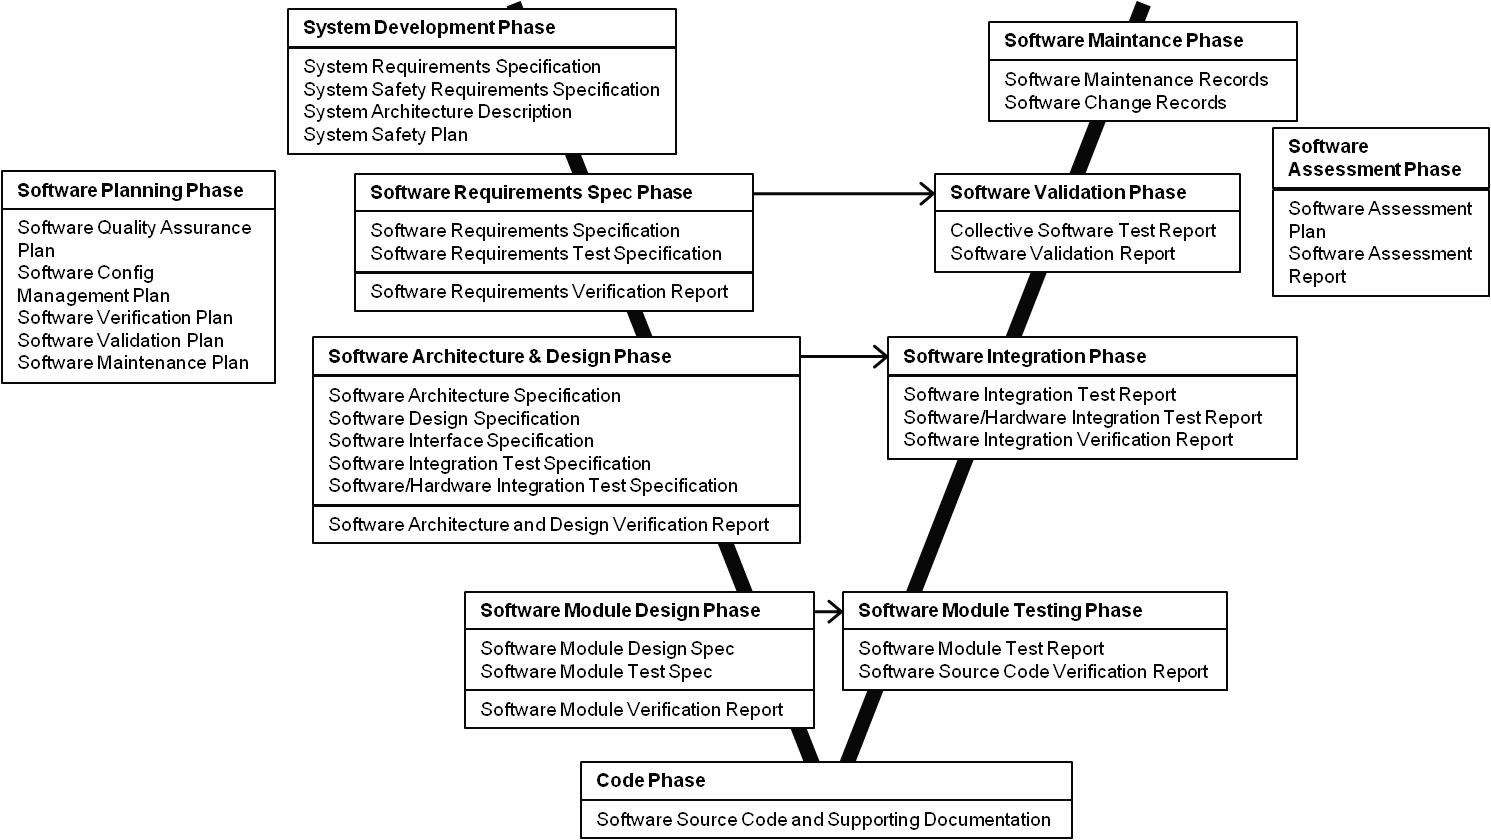
\includegraphics[scale=0.6]{Development-lifecycle-EN50128-own.png}
\caption{Recommended Development Lifecycle in EN 50128:2011}
\label{fig:Development-lifecycle-EN50128}
\end{figure}

On the base of this lifecycle the software development tool chain has to be able to provide assistance and generate all needed software and documents for all following eleven phases:

\vspace{-10pt}
\begin{enumerate} [topsep=2pt, partopsep=2pt,itemsep=2pt,parsep=2pt]
  \item System Planning and Development
  \item Software Requirements Specification
  \item Software Architecture and Design
  \item Software Module Design
  \item Code
  \item Software Module Testing
  \item Software Integration
  \item Software/Hardware Integration
  \item Software Validation
  \item Software Assessment
  \item Software Maintenance
\end{enumerate}

As the phase feature different tasks and related documents which have to be generated and used by a number of different persons in various roles a structured development process has to be applied. To be able to prove that all safety properties of the ETCS system are captured in the system requirements and software specifications, as well as that the final software product satisfies all specifications, a formal approach is necessary. As the scope of the openETCS project is to allow formal proof for the ETCS on-board software development, formal methods have to be used to provide the basis for formal proofs. 

Thereby formal methods is just a generic term for mathematical based procedures covering a number of different functionalities like notations, design techniques and software tools.  A more precise classification has to be used to distinguish the needed components and their requirements. We will use the BMW-Concept which separates between the following three means needed to handle tasks \citep{Schnieder.1999}:


\vspace{-10pt}
\begin{itemize}[topsep=2pt, partopsep=2pt,itemsep=2pt,parsep=2pt]
  \item \textbf{B}eschreibungsmittel (ger.): Means of Description (eng.),
  \item \textbf{M}ethoden (ger.): Methods (eng.) 
	\begin{itemize} 
	 \item Combination of a Means of description and a method represents a technique
	\end{itemize}
  \item \textbf{W}erkzeuge (ger.): Tools(eng.).
	\begin{itemize} 
	 \item Combination of a means of description, a method and a tool creates a technology
	\end{itemize}
\end{itemize}


The means of description is  the notation in which all artifacts are clearly modelled and from which a presentation of results can be generated. This can range from a natural language to highly mathematical languages \citep{Schnieder.2010}. Thereby the degree of formalisation for means of description can be classified  by their sigmatic,  logical syntax and semantic as it is shown in table \ref{tab:degree_of_form} \citep{Schnieder.2010}.

\begin{table}[htp]

\caption{Degree of formalisation for means of description}
\label{tab:degree_of_form}

\begin{tabular}{|m{0.6cm}|m{2cm}|m{2.5cm}|m{2.5cm}|m{2.5cm}|m{3cm}|}



\hline
 \multicolumn{2}{|c|}{} & \multicolumn{3}{|c|}{ Semiotic aspects of means of description} & \\ \hline
 \multicolumn{2}{|c|}{} & Sigmatic & logical syntax & semantic & Example \\ \hline

\multirow{3}{*}{\rotatebox{90}{~\parbox{6cm}{Degree of formalisation} }} & Informal & Incompletely defined set of symbols & Informal defined & Informal defined & Natural language \\ \cline{2-6}
 & Semi-formal & Completely defined set of symbols & In some cases mathematically defined to be unambiguous, complete and consistent   (often defined merely informal) & Informal defined & Message sequence charts and Structured analysis \\ \cline{2-6}
& Formal & Completely defined set of symbols & Mathematically defined to be unambiguous, complete and consistent & Mathematically defined to be unambiguous, complete and consistent  & Programming languages and Petri nets \\ \hline


\end{tabular}
\end{table}


 Every development process runs through a sequence of tasks with multiple iterations in between and various interactions between the different tasks. The methodology defines the way a tasks is handled by specifying the explicit result of the task and how it is reached. Furthermore to apply the methodology on a task by using the means of description a tool is needed. 

In the context of modern computer-based working processes tools are almost exclusively realized as software programs that are used to create system designs and immediately analyse them. 

In this way the integration of a suitable means of description (B),  the structured process of a methodology (M) and the support of an applicable tool (W) allows to distinguish three orthogonal means, which together provide the needed functionalities, but are independent from each other as far as they can be used separately and exchanged. In practice, a clear distinction between means of description and methodology is not always given, so that both are summarised under the term technique. To follow the structured system development approach of the CENELEC standards in an "open" way means of description, methods and tools have to be chosen, which can be used by everyone. 

The CENELEC standards do not demand the use of certain means of description, methods or tools, but give recommendations for all process steps and Safety Integrity Levels (SIL). But the standard requires the use of semi-formal and formal means of descriptions. Functionality and Black-Box tests are mandatory for verification and validation of software with SIL 3 and SIL 4 and highly recommended for lower levels. To validate the final software also performance tests are needed. A traceability of all requirements and specifications over all steps of the development process has to be guarantied according to the \citeauthor{EN50128:2011}. 

\chapter{Expert interviews}

The main source to receive information for this analysis of the existing means of description, methods and tools used for the  development of safety relevant railway and comparable systems have been interviews with experts from the railway sector and other  industries concerning their approaches and their experiences. Overall 14 interviews  with experts from different fields have been conducted  at the following companies:


\vspace{-10pt}
\begin{itemize}[topsep=2pt, partopsep=2pt,itemsep=2pt,parsep=2pt]
  \item AEbt (Germany)
  \item Alstom (France)  
  \item CERTIFER (Paris)
  \item DB Fernverkehr (Germany)
  \item DB Netz (Germany)
  \item ERTMS Solutions (Belgium)
  \item Formalmind (Germany)
  \item RATP (France)
  \item SNCF (France)
  \item Systerel (France)
  \item Siemens (France and Germany)
  \item SRE (Switzerland)
\end{itemize}

A number of interviews with other valuable experts were enquired but could not be realised due to scheduling problem.


\vspace{-10pt}
\begin{itemize} [topsep=2pt, partopsep=2pt,itemsep=2pt,parsep=2pt]
  \item Airbus (France)
  \item BMW (Germany)
  \item Bombardier (Germany)
  \item SBB (Switzerland)
  \item BAV (Switzerland)
\end{itemize}

The interviews have been carried out as a free conversation between the up to three interviewees and the usually two interviewers. Although the main focus for every interview has been chosen according to the company's field of business and the expertises of the interviewees, every interview was guided by the questionnaire presented in Appendix \ref{chap: questionnaire}, which focuses on the following six categories of questions:

\vspace{-10pt}
\begin{enumerate}[topsep=2pt, partopsep=2pt,itemsep=2pt,parsep=2pt]

	\renewcommand{\theenumi}{\Alph{enumi}}
	\renewcommand{\labelenumi}{\theenumi}

  \item Business and organization of the company
  \item Methodology, means of description and tools for there software system development process
  \item Methodology, means of description and tools used for source code generation
  \item Verification and validation processes for models and code
  \item Experiences with different methodology, means of description and tools
  \item Requirements on future methodology, means of description and tools
\end{enumerate}

As most  experts are only involved in a small part of the system development process individually not appropriate questions where skipped,  but in most interviews all six categories were covered. Subsequent to the interview the provided information were edited and analysed by the interviewers. If necessary, the interviewees have been asked to clarify certain answers or to provide additional information for further research. With this approach the interviews were able to provide a broad overview about methods, means of description and tools which are currently used.

An overview about all relevant means of description discussed during the interviews and their properties is given in Chapter \ref{chap: MoD}. The methods used for the development of safety relevant software systems and eventual constrains concerning their use in the openETCS project are presented in \ref{chap: methods}. Subsequently chapter \ref{chap: tools} introduces the tools used in practice to apply the means of description according to the methods.

Although to not limit the answers to a certain aspect the last questions concerning the requirements for future methodology, means of description and tools where designed in an open way. Nevertheless, most interviewees focused on tool characteristics. This is comprehensible as in practice  methodology and means of description are implied by the use of tools. As these tool requirements are indirectly connected to more general requirements for the methodology and the means of description a list of common requirements for all components has been established based on the interviews. These are presented in chapter \ref{chap: requirements}.
\FIXME{\em The reference to requirements ist shown in the pdf as ?? }

\chapter{Means of Description}

\label{chap: MoD}

In general it can be observed that documents formulated in natural language are ambiguous, since its syntax and semantics always provide room for interpretation for the communication partners. As the means of description provide the basic notations in which the different development task are handled, a wide range of different means of description have been developed to facilitate communication. In general, every mean of description is defined by its symbolism, syntax and semantics which are specified more or less detailed and formal \citep{Schnieder.2003, Schnieder.2010}.  

Depending  on the various circumstances under which means of description have been developed and their basic theoretical concepts various characteristics and attributes can be distinguished.  The following  criteria can be used to characterize  means of description based on the guideline \citeauthor{VDIVDE3681}:
\vspace{-10pt}
\begin{itemize}[topsep=2pt, partopsep=2pt,itemsep=2pt,parsep=2pt]
  \item Formal basis
  \item Representation
  \item Description of structure
  \item Description of behaviour
  \item Explicit time representation
\end{itemize}
Further more the applicability of all means of description in practical applications is influenced by the following three aspects:

\vspace{-10pt}
\begin{itemize}[topsep=2pt, partopsep=2pt,itemsep=2pt,parsep=2pt]
  \item Required expertise
  \item Level of standardisation
  \item Tool support
\end{itemize}

\FIXME{\em The criteria list should be extendet with deterministic behaviour. Some languages (example: SysML state machines) do not guarantee determinisc behavior of functions due to ambigious semantics. For safety related function determism is an indispensible criterium ! }

Corresponding with these criteria means of descriptions are suited to be used in different development phases. Overall the following for levels of abstraction have to be supported:

\vspace{-10pt}
\begin{itemize}[topsep=2pt, partopsep=2pt,itemsep=2pt,parsep=2pt]
  \item System development
  \item Software requirements and specifications
  \item Software architecture and design specifications
  \item Software source code and the compiled object code
\end{itemize}

Table \ref{tab:TabMoD-short2} gives an overview of the relevant properties of means of description and techniques used for system  and software development. Therefore also programming languages have been incorporated in this list, which are in general not seen as formal methods. As this list is based on the means of description discussed during the interviews, used in comparable project and the formal methods named in the CENELEC standards, it just provides examples and cannot be seen as complete. The criteria used in table \ref{tab:TabMoD-short2} are adopted from the \citeauthor{VDIVDE3681} and based on the important requirements for means of descriptions named during the interviews. The assessment for each means of description is based on the information provided during the interviews, the CENELEC standards and additional research. For that purpose the instructions manuals and  bibliographies of techniques were examined.


\begin{center}
   \begin{landscape}
%\begin{sidewaystable}
\begin{table}[htp]

\caption{Characterisation for relevant Means of Description in basis of  VDI/VDE 3681:2005}
\label{tab:TabMoD-short2}


\begin{tabular}{|m{6cm}|m{0.8cm}|m{0.5cm}|m{0.8cm}|m{0.8cm}|m{0.8cm}|m{0.8cm}|m{0.8cm}|m{0.8cm}|m{0.5cm}||m{0.8cm}|m{1.5cm}|m{1.5cm}|m{2cm}|}

\hline
 & \multicolumn{9}{|c|}{Criteria} & \multicolumn{4}{|c|}{ Level of abstraction} \\ \hline
& \rotatebox{90}{~\parbox{2.8cm}{MoD/Technique} }&
\rotatebox{90}{~\parbox{2.8cm}{Formal basis}}& 
\rotatebox{90}{~\parbox{2.8cm}{Representation}}&
\rotatebox{90}{~\parbox{2.8cm}{Description of structure}} &
\rotatebox{90}{~\parbox{2.8cm}{Description of behaviour}} &
\rotatebox{90}{~\parbox{2.8cm}{Explicit time representation}} &
\rotatebox{90}{~\parbox{2.8cm}{No expertise required}} & 
\rotatebox{90}{~\parbox{2.8cm}{Level of standardization}} &
\rotatebox{90}{~\parbox{2.8cm}{Tool support}} &
\rotatebox{90}{~\parbox{2.8cm}{System development}} &
\rotatebox{90}{~\parbox{2.8cm}{Software requirements and specifications}} &
\rotatebox{90}{~\parbox{2.8cm}{Software architecture and design specifications}} & 
\rotatebox{90}{~\parbox{2.8cm}{Software source code and the compiled object code}} \\ \hline
ACSL (ANSI/ISO C Specification Language) and C&MoD&o&T&+&+&-&-&+&+&&+&+&+ \\ \hline
Ada and Spark&MoD&o&T&+&+&-&-&+&+&&&+&+ \\ \hline
Alloy&MoD&+&M&+&+&-&-&-&+&o&+&+&\\ \hline
CNL (Controlled Natural Language)&MoD&+&T, M&-&o&-&o&-&o&o&+&& \\ \hline
HOL (High Order Logic)&MoD&+&M&+&+&+&-&-&o&o&+&& \\ \hline
Lustre/ Textual and graphical Scade&MoD&+&T, G&+&+&-&-&o&+&o&+&+&+ \\ \hline
OBJ&MoD&+&M&+&o&-&&&&&&& \\ \hline
Timed Petri Nets&MoD&+&M, G&+&+&+&-&+&o&+&+&& \\ \hline
Process Calculi (CCS, CSP, LOToS)&MoD&+&M&-&o&&&&&&&& \\ \hline
RSL (RAISE Specification Language)&MoD&+&M&+&+&+&-&o&+&o&+&+& \\ \hline
State Machines&MoD&+&M, G&-&+&-&-&-&+&+&+&& \\ \hline
TL (Temporal Logic)&MoD&+&M&-&+&-&-&-&o&&&+& \\ \hline
UML 2.0 (Unified Modelling Language) and SysML (System Modelling Language)&MoD&o&T, G&+&+&+&-&+&+&+&+&o& \\ \hline
VDM (Vienna Development Method)&Tech&+&M&+&o&-&-&+&+&o&+&+& \\ \hline
Z, B - Method and Event B&Tech&+&M, G&+&+&o&-&+&+&o&+&+& \\ \hline

\multicolumn{14}{|c|}{MoD - Means of Description, Tech - Technique; T - textual, M - mathematical-symbolic, G - graphical} \\
\multicolumn{14}{|c|}{+ - fulfills criteria completely  (can be used) , o - fulfills criteria partially (can be used to some extent), - - does not fulfills criteria (cannot be used)} \\ \hline

\end{tabular}
\end{table}

%\end{sidewaystable}
   \end{landscape}
\end{center}


From the means of description presented in  \citeauthor{EN50128:2011}  only UML, B-Method and Petri Nets were named during the interviews as actually used means of description for modeling the requirement specifications and developing the software architecture and design. In addition State machines and Lustre/ Textual Scade are commonly used for software development. C and ADA and their related languages are primary used as programming languages to write the source code. Therefore these set of means of description can be seen as proven in use for the current software development. The following subsections present further information for every means of description. A more detailed version of the characterisation table is given in Appendix \ref{chap: TabMoD}.

\section{UML 2.0 (Unified Modelling Language) and SysML (System Modelling Language)}


	\textbf{Characteristics}

	The Unified Modelling Language (UML) an the System Modelling Language (SysML) are object-oriented means of description specified by the Object Modelling Groupe (OMG). Both consist of a number of different diagrams to describe the various aspects of a system. Thereby SysML can be understood an extension of a certain subset of UML developed for system engineering as it uses a part of the UML diagrams. In addition both languages interchanged their models using the XML Metadata Interchange (XMI) standard defined by OMG. Respectively a number of tools are developed to work with both languages.

	\textbf{Typical applications}


	\textbf{Standards}


	\textbf{References}

Links:

\url{http://www.uml.org/} \\[4pt]
\url{http://www.omgsysml.org/}\\[4pt]
\url{http://www.omg.org/} \\[4pt]

Bibliography:

Weilkiens, Tim. \textit{Systems Engineering with SysML/UML: Modeling, Analysis, Design}. Morgan Kaufmann / The OMG Press, Boston,  2007.\\[4pt]
Ambler, Scott William. \textit{The Object Primer: Agile Model Driven Development with UML 2}. Cambridge University Press, Cambridge, 2004.\\[4pt]

\section{Petri Nets}


	\textbf{Characteristics}


	\textbf{Typical applications}


	\textbf{Standards}


	\textbf{References}

Links:



Bibliography:




\section{Z, B - Method and Event B}


	\textbf{Characteristics}


	\textbf{Typical applications}


	\textbf{Standards}


	\textbf{References}

Links:



Bibliography:

\section{Lustre/ Textual and Graphical Scade}

	\textbf{Characteristics}

SCADE is a formal modelling language targeted for safety-critical embedded control applications in the avionics, rail, automotive and industrial automation domain. SCADE source code can be written as text (for anyone who likes writing plain text) or (more usual) as schematic diagrams. SCADE models are synchronously clocked data flow and state machines, that can be nested and intermixed with each other without limitations. 
SCADE provides DO-178B- and EN50128-certified code generators producing C or ADA code as output. SCADE models are therefore concrete, deterministic, executable and verifiable; it allows the production of rapid prototype as well as of safety related target system software. 

	\textbf{Typical applications}

Safety critical systems like
\vspace{-10pt}
\begin{itemize}[topsep=2pt, partopsep=2pt,itemsep=2pt,parsep=2pt]
  \item Rail interlocking systems
  \item Rail track vacancy detection systems
  \item Rail train control systems
  \item Rail Level-crossing protection systems
  \item Avionic flight controller
\end{itemize}


	\textbf{Standards}


	\textbf{References}
	
\url{http://www.mobility.siemens.com/mobility/global/en/interurban-mobility/rail-solutions/rail-automation/Pages/rail-automation.aspx/} \\[4pt]	

Links:

\url{http://esterel-technologies.com/} \\[4pt]
\url{http://www.interested-ip.eu/}\\[4pt]
\url{http://http://www.interested-ip.eu/final-report.html/} \\[4pt]


Bibliography:

\section{State Machines}


	\textbf{Characteristics}


	\textbf{Typical applications}


	\textbf{Standards}


	\textbf{References}

Links:



Bibliography:

\section{VDM (Vienna Development Method)}


	\textbf{Characteristics}


	\textbf{Typical applications}


	\textbf{Standards}


	\textbf{References}

Links:



Bibliography:

\section{Process Calculi (CCS, CSP, LOTUS) }


	\textbf{Characteristics}


	\textbf{Typical applications}


	\textbf{Standards}


	\textbf{References}

Links:



Bibliography:

\section{HOL (High Order Logic)}


	\textbf{Characteristics}


	\textbf{Typical applications}


	\textbf{Standards}


	\textbf{References}

Links:



Bibliography:

\section{DSL (Domain Specific Languages)}


	\textbf{Characteristics}


	\textbf{Typical applications}


	\textbf{Standards}


	\textbf{References}

Links:



Bibliography:

\section{TL (Temporal Logic)}


	\textbf{Characteristics}


	\textbf{Typical applications}


	\textbf{Standards}


	\textbf{References}

Links:



Bibliography:

\section{OBJ}


	\textbf{Characteristics}


	\textbf{Typical applications}


	\textbf{Standards}


	\textbf{References}

Links:



Bibliography:

\section{CNL (Controlled Natural Language)}


	\textbf{Characteristics}


	\textbf{Typical applications}


	\textbf{Standards}


	\textbf{References}

Links:



Bibliography:

\section{Alloy}


	\textbf{Characteristics}


	\textbf{Typical applications}


	\textbf{Standards}


	\textbf{References}

Links:



Bibliography:

\section{Ada and Spark}


	\textbf{Characteristics}


	\textbf{Typical applications}


	\textbf{Standards}


	\textbf{References}

Links:



Bibliography:

\section{ACSL (ANSI/ISO C Specification Language) and C}


	\textbf{Characteristics}


	\textbf{Typical applications}


	\textbf{Standards}


	\textbf{References}

Links:



Bibliography:

\section {RSL (RAISE Specification Language)}


	\textbf{Characteristics}


	\textbf{Typical applications}


	\textbf{Standards}


	\textbf{References}

Links:



Bibliography:


\section{Summary}

This selection of various means of description used in the railway industry shows that the notations have been developed with different targets so there is probably no single means of description able to support all levels of abstraction and to describe all structural and behavioural aspects of a system. Therefore a combination of means of description is needed to support all development steps and to capture all aspects of an ETCS on-board system. The advantages of using different means of description for an easier understanding or a more exact notation of certain aspects have to be evaluated against the difficulties of coordinating the different means of description. To ensure consistency over all levels of abstractions when means of description are changed the area of use for every means of description has to be clearly defined and validated automatic translation should be used.  Overall the chosen means of description has to provide the needed formal notation to apply the methodology. 



\chapter{Methods}

\label{chap: methods}

Usually one methodology is used to handle one step in the development process. If a methodology can cover only a certain aspect of a development step certain methods can be combined. The Appendix A of \citeauthor{EN50128:2011} lists a number of methods for every step of the software development life cycle and gives recommendations which methods  to use. Especially for the verification an validation steps combinations of methods are necessary. According to the standards the software requirements specification have to be provided  in natural language and if necessary in a formal/ semi-formal description. 

As the openETCS project looks for methods to incorporate the open proof approach into the software development  for the ETCS on-board unit, the  characteristic of proofability has to be considered for all determined software requirements. Since  the system requirements specifications are provided in a textual way, these have to be translated into a formal description to allow for mathematical reasoning and to establish proofable software specifications. During the development this formal description has to be translated back into natural language to provide all kinds of needed documentation. Overall suitable methods for the following seven general functionalities of the software development process have to be found:

\vspace{-10pt}
\begin{itemize}[topsep=2pt, partopsep=2pt,itemsep=2pt,parsep=2pt]
\item Transformation of textual specifications in formal specifications
\item Transformation of formal requirement specifications in formal software and software module design and architecture descriptions
\item Source code generation
\item Verification of models and source code
\item Validation
\item Creation of documentation
\item Terminology management/Intelligent Glossary
\end{itemize}

The interviews have shown that these tasks are normally divided in a number of subtasks according to the used methodology. Respectively a broader methodology defines the  process to deal with the task and more specific methods describe the actual work steps. This approach is backed through the recommendations given in the \citeauthor{EN50128:2011}. The following sections present the methods applied in practice to handle the six general tasks.

\section{Transformation of textual specifications in formal specifications}

As a formal specification is build using a formal mean of description, their properties mainly defines the actual process to translate the natural language requirements into a formal notation. Thus, this task is usually handled by experts who are familiar with the formal means of description and try to formulate the formal description as the read the textual specification. As this process depends on the individual knowledge and understanding of the expert the interviews have not been able to cover those work steps in all details. But in generically the two following subtasks had to be completed for every textual requirement to provide a complete formal model:
\begin{itemize}
\item Informal analysis: Collect and categories the requirements stated in text
\item Formalization: Allocated the category of requirement to a concrete formal representation and put these in relation to all other already formalised requirements
\end{itemize}

In some case a generic list of specific categories of requirements and their allocated concept of formal representation have been established at the beginning, but mostly these steps are done more or less consciously during the translation. 

The methodology described in \citep{Cimatti.2008c} can be seen as representative way how the textual system requirement specifications covered in subset 26 can be translated systematically into a formal/semi-formal description. In this case the chosen methodology is based on UML diagrams combined with CNL, which allows subsequently to verify the formal specification through model checking.

During the informal analysis step the textual specifications are decomposed in basic requirements which are collected using an appropriate tool to store them. These basic requirements can then be classified by assigning one of the eight categories from table \ref{tab:categories of requirements}.

\begin{table}[h]

\caption{Categories of requirements according to \citep{Cimatti.2008c}}
\label{tab:categories of requirements}

\begin{tabular}{|p{4.5cm}|p{9.3cm}|}
\hline
\textbf{Category}  &  \textbf{Description} \\ \hline
Glossary & Defines a particular term/concept \\ \hline
Architecture &  Introduces some system's modules and their interactions \\ \hline
Functionality/behaviour & Describes the behaviour a module can perform or the states a module can be in \\ \hline
Communication &  Describes massages exchanged between modules \\\hline
Environmental &  Describes constrains on the model \\\hline
Scenario & Describes possible scenario \\\hline
Property &  Describes expected/required properties \\\hline
Annotation & Notes in the specification\\
\hline
\end{tabular}

\end{table}

Afterwards the basic requirement is expressed by using the associated UML or CNL formalisation which is linked back to the textual requirement  to provide traceability. The methodology in \citep{Cimatti.2008c} for example uses UML state machines to  formalise  functional/behavioural requirements and CNL to specify environmental requirements. 

Independent of the concrete methodology and the used means of description the interviews have shown that it is central to guarantee the traceability of all requirements as the completeness of the software can only be validated if it is documented that the entire textual specification is covered. Therefore the traceability has to be established from the source code to the formal specifications and from there back to the textual specifications. Differences between the textual and the formal specification have to be reasoned by linking it to  inconsistencies or incompleteness in the textual specifications. 


\section{Transformation of formal requirement specifications in formal software and software module design and architecture descriptions}

To write their formal software requirement specifications and to define the software architecture and design based on these most organisations presented a model-based development process using different formal models to describe the software on different abstraction levels. In doing so the railway operators mostly focus on the high-level description of system and software functionality, while the actual software developers concentrate on modeling the more concrete software architecture and design. By using formal methods and formal refinement certain steps of the top-down modeling can be automated. Since every organisation used a modular approach as it is mandated by \ref{EN50128:2011} for all SIL Levels the refinement is also used to separate the functionalities of different modules. Thereby the detailed software model can than be used for an automatic or semi-automatic source code generation. To model the interactions with adjacent systems including human operators a model representing the environment is needed. Overall our interviews have confirmed that a variation the top-down model-based software development shown in figure \ref{fig: MBD} is common practice at least for the development of safety related software. 

\begin{figure}[h]
\centering
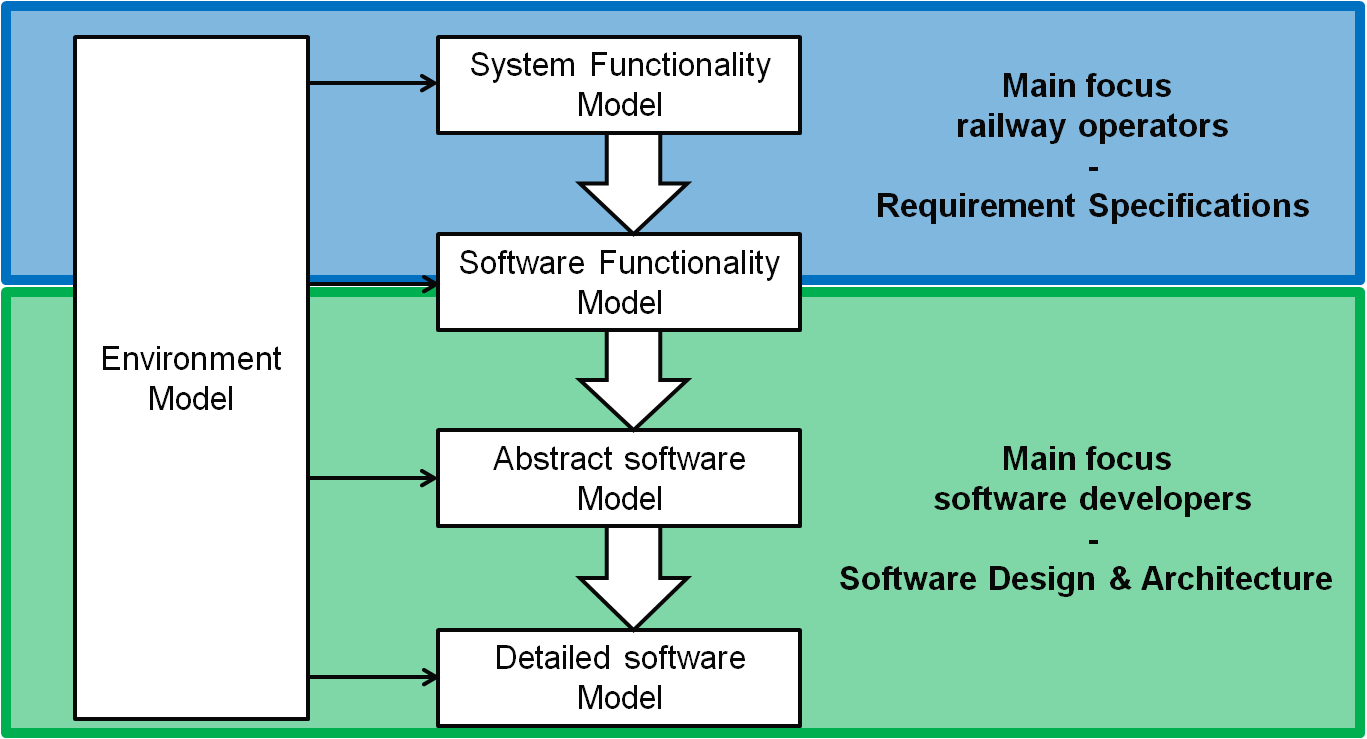
\includegraphics[scale=0.6]{Model-based_Approach.png}
\caption{Model-based development approach for software development}
\label{fig: MBD}
\end{figure}

To guarantee certain modeling standards all organisations had defined training processes for their experts which introduced them to certain modeling standards building the mutual basis for all models.  Additionally most organisations use models that can be analysed and/or simulated during the modeling process to receive feedback from these methods about certain properties of the model during their model-based development process.

It has already been shown in chapter \ref{chap: MoD} usually different means of descriptions are used to build functionality models than design and architecture models. As most organisations are focus either on high-level functional models or on design and architecture models they use only one means of description for all models in their internal model-based development process. But usually functionality models which are handed done in the development process for example from an operator or train manufacturer to the software developer have to be translated. Therefore a dependable translation methodology is needed to ensure that all functionalities are incorporated in the software models and to guarantee traceability over all levels of abstraction. In practical applications this is mostly handled by validated translation tools and though corresponding test cases.

\section{Source code generation}

Using the model-based development approach most interviewed organisations generated source code based on their software design and architecture models. As the  methodology for source code generation depends explicitly on used means of description and programming language the interviews have not been able to cover them in detail. Especially as most commercial modeling tools for UML, B-Method, SCADE and Simulink already provide an incorporated methodology for automatic code generation. 

In most cases ADA and C and their related programming languages are used for source code generation. The source code is then compiled into executable software, in doing so the compiler has to be validated to guarantee that the software behaviour is according to the source code definition.

Another methodology to implement the functionality expressed in a model into a software is to use an interpretor .

The interpretor is a generic software build to understand the functionality of a certain kind of model which then hands the commands created in the executable model directly down to the hardware controls. Therefore the functionality can be change by just exchanging the model with any changes at the interpretor. To guarantee that the interpretor can provide the wanted functionality he has to understand every possible model behaviour and to convert this into all required commands. Like every used translator or compiler the interpretation has to be validated to ensure a dependable execution.

This methodology which absolutely separates functionality and lower level control parts is currently used for interlocking-systems to guarantee a manufacturer independent programming of functional rules. In this process a specific kind of Petri net models is used to describe the needed system behaviour for every interlocking. If a new behaviour is required only the Petri nets model has to be modified.

As such processes of formal automatic source code generation or model interpretation requires a large effort and completely validated tools this methodology is in the majority of cases only used for safety relevant software.  For non-safety relevant software semi-formal code generation is mostly applied to reduce the costs even if this usually creates more bugs. 

\section{Verification of models and source code}

To verify the different models and the source code basically to groups of methods can be used:
\vspace{-10pt}
\begin{itemize}[topsep=2pt, partopsep=2pt,itemsep=2pt,parsep=2pt]
\item Formal analysis and proof
\item Testing
\end{itemize}

While testing reasons that the required defined properties are present when the model or the software  shows the wanted behaviour in a number of scenarios, formal analysis and proof use the formal basis of the means of description to reason that the stated properties cannot be violated by the model or source code. Accordingly the formal methods can only be applied if  model or source code are formal and the properties, which have to be verified are stated in a formal description. 

The properties a system has can be distinguish into the following to categories:

\vspace{-10pt}
\begin{itemize}[topsep=2pt, partopsep=2pt,itemsep=2pt,parsep=2pt]
\item State/Transition properties,
\item Functional properties,
\item Structural properties,
\item Behavioural properties. /citep{Schnieder.2010b}
\end{itemize}

Suitable methods have to be chosen to verify all four kinds of properties. 

Generally formal proof, testing and simulation are general principals covering a number of more concrete methods, which have to be chosen concerning the specific properties that have to be verified through the principal.

\subsection{ Formal analysis and proof}

Since formal proofs are able to demonstrate the general existence of a property based on mathematical reasoning, a formal proof is able to replace testing if it can be applied. Correspondingly, the interviews have shown that it is already common practice for train control systems to verify the software design and architecture almost exclusively through formal proof as it is illustrated in figure \ref{fig: MBD-Formal-Proof}.

\begin{figure}[ht]
\centering
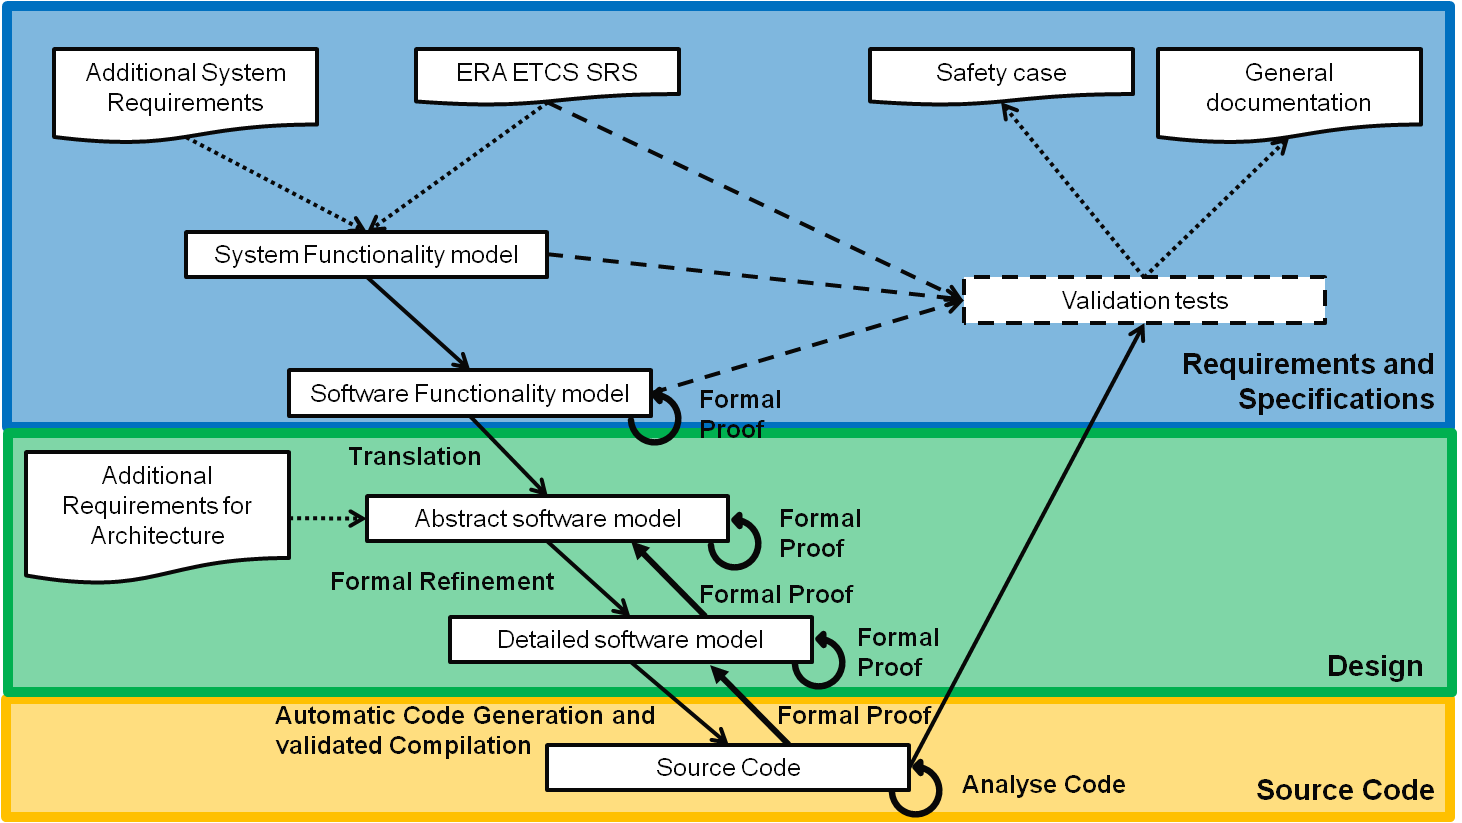
\includegraphics[scale=0.6]{Lifecycle-Model-based-Approach-Formal-Proof.png}
\caption{Model-based development with verification through Formal Proof and additional Testing for validation}
\label{fig: MBD-Formal-Proof}
\end{figure}

To apply formal analysis and proof basically three different methods can be used: 

\vspace{-10pt}
\begin{itemize}[topsep=2pt, partopsep=2pt,itemsep=2pt,parsep=2pt]
\item Theorem Proving,	
\item Model Checking, and
\item Simulation.	
\end{itemize}

As a theorems is a mathematical statement which has to be proven based on the basis of certain assumptions theorem proving as a methodology able to verify properties also for infinite systems. Respectively, the ability to prove a theorem is based on the mathematical system description which implies that there can be cases in which a theorem can neither be proven nor disproved. Therefore in some cases it is necessary to adopted the formal description to make certain properties provable.

Model checking uses the formal structure of a model to prove that certain states or variable values which are connected to certain properties can or can not be reached. Therefore the model-based description is limited to a finite number of system states. If a property is rejected a counterexample is provided.

If the mathematical description of all specifications can be simulated it is possible to analyses the system properties according to possible inputs. This can be used to proof, that under all inputs the system shows the required properties. Usually this is used to show certain behavioural properties.

In general  formal analysis and proof can only be applied for properties which can be stated in a formal way that is consistent with the mathematical theory used for the underlying model description. This can be challenging if abstract properties shall be proven for a detailed software design. Therefore the interviewees using formal prove for their software verification emphasised especially that the main part of the work is to define the properties to prove and to refine them for every abstraction level.

\subsection{Testing}

Test methods range from simple checklists to highly complicated Test scenarios. To verify by test that a model fulfills certain requirements a tests cases have to generated which describe what has to be done during the tests and which result is expected. As for complex systems test cases can never cover all possible scenarios testing cannot provide a full guarantee that a properties holds under all circumstances.

Tests can be a static analysis which just ensures that certain aspects are covered by the model or source code or it can be a dynamic test which sets some starting conditions and expects that the model or code  responds in a certain way. The simplest kind of dynamic tests are Funtional/Black-Box Tests which just specify inputs and expected outputs without any information about the  actual system structure. These are mandatory for the verification of SIL 3 and SIL 4 software, but can be enhanced trough a more precise test case specification as more are available.

These test cases can be modeled by an expert based on the modeled or textual requirements that should be verified or they could be generated in a automatic way based on a formal requirement model. As most organisations we have interviewed use a model-based development for their software development those how used testing for verification applied model-based testing by simulation of their models and creation of test cases based on these models. Figure \ref{fig: MBD-Testing} shows the process structure for a model-based development process with testing for verification and validation.

\begin{figure}[h]
\centering
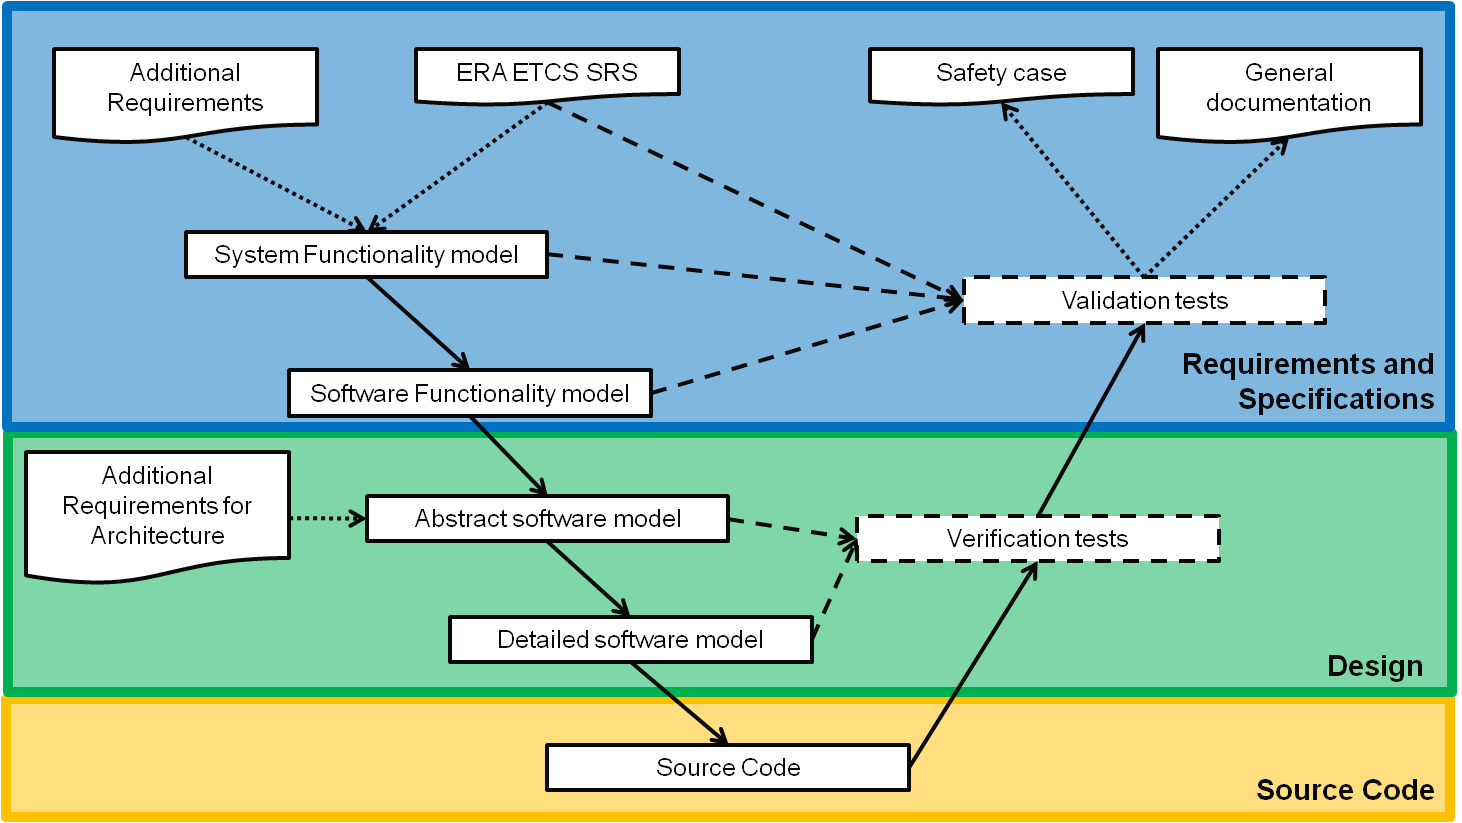
\includegraphics[scale=0.6]{Lifecycle-Model-based-Approach-Testing.png}
\caption{Model-based development with verification and validation through testing}
\label{fig: MBD-Testing}
\end{figure}

In general test cases are collected in catalogue against which every new version of the model or code is tested. To reduce the amount of work this is usually automated by using a test environment which combines the test case catalogue with an execution tool and provides a test report at the end.

\section{Validation}

Asked for the validation methodology the interviewed organisations explained that the following three methods are mandatory for validation according to \citeauthor{EN50128:2011}:

\vspace{-10pt}
\begin{itemize}[topsep=2pt, partopsep=2pt,itemsep=2pt,parsep=2pt]
\item Traceability for functional and non-functional Requirements
\item Functional/Black-Box tests
\item Software performance tests
\end{itemize}

As verification and validation are closely related in product development most organisations which used formal proof for verification also this methodology for tasks in their validation process. But as validation has to refer back to the original textual system requirements as every organisation we interviewed argued it can not be done entirely by formal proof. Accordingly a combination of tests and formal analysis and proof is used by these organisation to validate their software as it shown in figure \ref{fig: MBD-Formal-Proof}. 

Overall the model-based development process itself already provides an important methodology validate the software against it requirements. The core of every validation process presented during the interviews has been modeling combined with traceability of all requirements from the original textual system specifications and a suitable catalogues of test cases created based on this textual specifications and their formal models.

\section{Creation of documentation}

Since the software development requires supporting documentation for operation, maintenance as well as for all safety related activities it is important to use a methodology the way all these documents are created. This involves not only a structure when and how documents are created and used which is mainly specified by CENELEC standards but also a methodology how the formal/semi-formal software descriptions are included into the documentation. As natural language documents a methodology is needed which that formal/semi-formal documents and textual documents are consistent.

Most organisations we interviewed already use tools which can automatically create documents based on their formal/semi-formal models. Usually these documents list the processes modeled including their input and outputs and some important modeling characteristics. If possible graphical representations of those models are added to illustrated the modeling work and provide additional information.

As the kind of information, which have to be extracted from specific models for a proper documentation can at least to a certain degree be universally determined it is common practice to 
create some parts of the textual documents automatically. Especially UML diagrams allow to incorporate specific variables from a diagram into a text by using predefined textual building blocks. This guarantees that the documentation is consistent with the model-based development activities and helps to reduce the needed amount of work to create the documentation as human editing is only needed to check the comprehensibility and to add parts in natural language that cannot be created from the models.

\section{Terminology management/Intelligent Glossary}

The used terminology has a central role in a development process to ensure that all participants understand the requirements in the same way and that these requirements a threated consistently during the whole development process \citep{Schnieder.2010}. To provide an overview about the specific terminology used to describe a system it is common practice to establish a glossary and a collection of abbreviations which provide definitions for most of the specific terms. Usually this glossary is just an additional documents for the textual system requirement specifications, which just provides a short explanation for every key term regarding to the concept that term is used in the requirement specifications. 

Some interviews emphasized to ensure a consistent terminology over all models and all process participants the relations between different terms have to be modeled, too, and these model has to be link to all models and documents to provide the right terminology to every process step, to allow additions and to provide a traceability over all abstraction levels. Some tools, especially those using UML or SysML, provide some a way to model the terminology and to connect it to other kind of models but no organisation we interviewed used a methodology providing all features of an intelligent glossary for the whole development process. The \textit{iglos} methodology which has been developed in an academic context can be used to clearly separate the meaning of terms in different domains and to allocated them so certain applications. Different kinds of relations can be modeled and the terms can be linked to sources and applications in the textual documents or the modeled system descriptions.

Overall the model-based development process requires an terminology managements methodology which provides the functionality of an advanced glossary gathering, handling and providing a systematic structure for the terminology to all parts of the development process. Therefore the used methodology has to be aligned with all means of descriptions, methods and tools used during the development process. 

\section{Summary}

Overall the interviews and the additional research have shown, that model-based approaches are common for all kind of safety relevant software development processes. Thereby some organisations already use such formal models to predominately verify their software design and architecture through formal proof. However, for validation a combination of formal proof and different testing methods is needed as formal proof can only been used for properties which can be state in a suitable way. A tabular overview about all presented methods is shown in appendix \ref{chap: Methodology}. The following chapter \ref{chap: tools} presents the tools used in practice to apply these methodology by making use of the different means of descriptions named in chapter \ref{chap: MoD}.


\chapter{Tools}

\label{chap: tools}

As it has already been described the tools are closely connected to a means of description  and a methodology which they support. Therefore a large number of different tools from various backgrounds are available which mostly handle on means of description and allow to apply one or more methods for different steps in the development process.

The interviews have shown that there are tools available and in use to support the following development steps and the connected methods depending on the general development process:

\vspace{-10pt}
\begin{itemize}[topsep=2pt, partopsep=2pt,itemsep=2pt,parsep=2pt]
\item Formalisation of textual requirements
\item Modelling

	\begin{itemize}
	\item System/software structure
	\item System/software behaviour
	\item Software architecture and design
	\end{itemize}

\item Formal refinement
\item Model translation
\item (Automatic) Code generation and compilation
\item Formal Proof

	\begin{itemize}
	\item Theorem proving
	\item Model checking (different levels)
	\item Simulation
	\end{itemize}

\item Analysis of source code
\item Testing

	\begin{itemize}
	\item Test environment (for model and software tests)
	\item Test case generation and test case database
	\end{itemize}


\item Traceability of requirements
\item Versioning and configuration management
\item Terminology Management
\item Documentation
\end{itemize}

Since the functionalities tools support can be used in different methods and for different development steps the use of a tool can be necessary at different times during the product lifecycle. Additionally some tools are able to provide a range of functionalities so they can be used to combine different methods. Accordingly it is  often difficult in practical applications to clear distinguish between tool functionality and supported methodology. Therefore most of the interviewees have focused on the main tools there are using for their model-based development and directly linked the tool to a step of their development process. An overview about the tools discussed during the interviews or presented in related publications is given in table \ref{tab: Tools}. The table also shows the development task which are supported by these tools . This table only covers the main tools named as relevant for the open ETCs project. Most tool developers provide a number of additional tools which interact with the main tool to provide a range of functionalities. These tools are not listed separately to keep the table focused on main tools.

%\begin{sidewaystable}

 \begin{landscape}
 \begin{center}

\begin{longtable}{|m{2.5cm}|p{3cm}|m{1.8cm}|p{3.5cm}||m{1.2cm}|m{0.2cm}|m{0.2cm}|m{0.2cm}|m{0.7cm}|m{0.2cm}|m{0.7cm}|m{0.2cm}|m{0.6cm}|m{1.2cm}|m{0.2cm}|m{0.2cm}|}

\caption{Overview of Tools and the support development processes}
\label{tab: Tools}\\

\hline Tool & Developer & License status & Means of Description & \begin{sideways} {~\parbox{3cm}{Formalisation of textual requirements}}\end{sideways} & \begin{sideways} {~\parbox{3cm}{Modelling}} \end{sideways}& \begin{sideways} {~\parbox{3cm}{Formal Refinement}} \end{sideways} & \begin{sideways} {~\parbox{3cm}{Model translation}} \end{sideways} & \begin{sideways} {~\parbox{3cm}{Code generation and compilation}} \end{sideways} & \begin{sideways} {~\parbox{3cm}{Formal Proof}} \end{sideways} & \begin{sideways} {~\parbox{3cm}{Analysis of source code}} \end{sideways} & \begin{sideways} {~\parbox{3cm}{Testing}} \end{sideways}  & \begin{sideways} {~\parbox{3cm}{Traceability of requirements}} \end{sideways} & \begin{sideways} {~\parbox{3cm}{Versioning and configuration management}} \end{sideways} & \begin{sideways} {~\parbox{3cm}{Intelligent glossary}} \end{sideways} & \begin{sideways} {~\parbox{3cm}{Documentation}} \end{sideways} \\ \hline
\endfirsthead

\hline Tool & Developer & License status & Means of Description & \begin{sideways} {~\parbox{3cm}{Formalisation of textual requirements}}\end{sideways} & \begin{sideways} {~\parbox{3cm}{Modelling}} \end{sideways}& \begin{sideways} {~\parbox{3cm}{Formal Refinement}} \end{sideways} & \begin{sideways} {~\parbox{3cm}{Model translation}} \end{sideways} & \begin{sideways} {~\parbox{3cm}{Code generation and compilation}} \end{sideways} & \begin{sideways} {~\parbox{3cm}{Formal Proof}} \end{sideways} & \begin{sideways} {~\parbox{3cm}{Analysis of source code}} \end{sideways} & \begin{sideways} {~\parbox{3cm}{Testing}} \end{sideways}  & \begin{sideways} {~\parbox{3cm}{Traceability of requirements}} \end{sideways} & \begin{sideways} {~\parbox{3cm}{Versioning and configuration management}} \end{sideways} & \begin{sideways} {~\parbox{3cm}{Intelligent glossary}} \end{sideways} & \begin{sideways} {~\parbox{3cm}{Documentation}} \end{sideways} \\ \hline
\endhead

\multicolumn{16}{|c|}{+ - can be used , o - can be used to some extent} \\
\multicolumn{16}{|r|}{{Overview of Tools and the support development processes - Continued on next page}} \\ \hline
\endfoot

\multicolumn{16}{|c|}{+ - can be used , o - can be used to some extent}\\
 \hline
\endlastfoot

Alloy 4&Software Design Group at MIT&free &Alloy&&+&+&&+&+&&&&+&&o \\ \hline
Artisan Studio&Atego&commercial&SysML und UML 2.0&o&+&&+&+&&&&+&+&o&+ \\ \hline
Atelier B&ClearSy System Engineering&free &B, Event B&&+&+&+&+&+&&&&+&&o \\ \hline
CompoSys&ClearSy System Engineering&commercial&Event B&o&+&&&&+&&+&&+&o&+ \\ \hline
Control Build&Geensoft&commercial&&&+&&&+&&&+&&+&&o \\ \hline
CPN&Eindhoven University of Technology&open source&Petri Nets&&+&&&&+&&+&&+&&o \\ \hline
Enterprise Architect&Sparx System&commercial&SysML und UML 2.0&&+&&&+&&&+&+&+&&+ \\ \hline
ERTMS FormalSpecs&ERTMS Solutions&open source&DSL&&+&&+&+&&&+&+&+&&o \\ \hline
Frama-C&CEA-LIST and INRIA-Saclay&open source&C&&&&&&+&+&&&&&o \\ \hline
iglos&TU Braunschweig, iVA&free/ commercial&Mult. MoD&+&&&&&&&&+&+&+&+ \\ \hline
iLock/iCertifier&Prover Technology AB &commercial&&&+&&+&+&+&+&+&&+&&+ \\ \hline
KNOW Enterprise&KnowGravity Inc.&commercial&UML 2.0 (xUML)&o&+&&+&+&&&+&+&+&o&+ \\ \hline
MagicDraw&No Magic&commercial&SysML und UML 2.0&o&+&& &+&&&+&+&+&&o \\ \hline
mCRL2&Technische Universiteit Eindhoven&free&mCRL2&&+&+&&&+&&&&+&&o \\ \hline
Modelio&Modeliosoft&open source&SysML und UML 2.0&o&+&&&+&&&o&+&+&&o \\ \hline
NuSMV&Fondazione Bruno Kessler&open source&BDD and SAT&&&&&&+&&&&&&o \\ \hline
Papyrus&CEA&open source&SysML und UML 2.0&+&+&&&&&&+&+&+&&o \\ \hline
Perfect Developer&Escher Technologies Ltd.&commercial&&&+&&&+&+&&+&&+&&o \\ \hline
PRISM&University of Oxford&open source&BDD and MTBDD&&&&&&+&&&&&&o \\ \hline
ProB&Formal Mind GmbH&open source&B&&&&&&+&&+&&+&&o \\ \hline
ProR&Formal Mind GmbH&open source&ReqIF 1.0.1&+&&&&&&&&&+&&+ \\ \hline
Rational Architect&IBM&commercial&SysML und UML 2.0&+&+&&+&+&&&+&+&+&&+ \\ \hline
SCADE Suite &Esterel Technologies S.A.&commercial&Lustre / Data Flow (Logic) + State machines&&+&+&+&+&+&+&+&+&+&&+ \\ \hline
Simulink/ Design Verifier&MathWorks&commercial&Block diagramms&&+&+&+&+&o&&+&&+&&o \\ \hline
SPARK GPL/ GNATprove&AdaCore&open source&Spark ADA&&+&&&+&+&+&+&&+&&o \\ \hline
SPIN&Bell Labs&open source&PROMELA&&&&&&+&+&+&+&&&o \\ \hline
$\pi$-Tool&IQST&commercial&Petri Nets&&+&+&+&&+&&+&&+&&o \\ \hline

\end{longtable}

\end{center}
\end{landscape}
%\end{sidewaystable}

The focus of the tool discussion during the interviews has been on modeling tools as the collection of tools in table \ref{tab: Tools} shows. Most companies use commercial tools like Artisan Studio, Atelier B,  Rational Architect,  SCADE or Simulink to build their software models by using the implemented means of description and the implemented methods to generate reliable source code in C or ADA languages. 

To use formal proof for these models usually on of the available commercial tools which fits to the modeling tool is chosen and than customised to a degree that it provides all needed functionalities. Usually this is handled in cooperation with the tool developer. Some companies have a lot of experience with tools for modeling and model proofing and therefore mainly handle the customisation in house.

But especially for proofing and source code analysis a large number of open source tools exist which usually have an academic background. Therefore most of them are not certified. But as some of these tools have been around for quite some time, they could be suitable to fulfill all requirements according to the CENELEC standards. As most interviewees confirmed open source software combined with support through a external partner could provide the needed level of customisation and service support required from most companies. Nevertheless most interviewees raised issues that it could be difficult to get broadly accepted and qualified tools for formal proof and code generation as open source products. Since there is a number of open source tools available for all task in the development process an in deeps evaluation is needed. 

The following sections will give a short introduction of every main tool presented as relevant during the interviews and the additional research. 

\section{Alloy 4}


	\textbf{Developer}

	Company: 

	Webside:

	Contact address:

	Other  Participators:



	\textbf{Typical applications}

	Field of usage:

	%Brief introduction to what the tool does

	%Applicability
	%Key capabilities
	Input:

	Output:

	% Main restrictions e.g. only a subset of the target language is covered

	% Manual or automated use of the tool e.g. which steps are manual and automatic in the use of the tool.

	% Expertise level e.g. which prerequisite is needed to use the tool


	Integration in a tool chain
	%Currently distributed: Yes/No
	%Underlying technologies E.g. Framework, .NET vs. Java, etc.

	%Describe equirement to install/run the tool (all that is necessary to make the tool work fine: OS, Java version, dependencies with other tools, Eclipse version, ...)


	\textbf{License}


	\textbf{References}

	Bibliography:





\section{Artisan Studio}

	\textbf{Developer}

	Company: 

	Webside:

	Contact address:

	Other  Participators:



	\textbf{Typical applications}

	Field of usage:

	%Brief introduction to what the tool does

	%Applicability
	%Key capabilities
	Input:

	Output:

	% Main restrictions e.g. only a subset of the target language is covered

	% Manual or automated use of the tool e.g. which steps are manual and automatic in the use of the tool.

	% Expertise level e.g. which prerequisite is needed to use the tool


	Integration in a tool chain
	%Currently distributed: Yes/No
	%Underlying technologies E.g. Framework, .NET vs. Java, etc.

	%Describe equirement to install/run the tool (all that is necessary to make the tool work fine: OS, Java version, dependencies with other tools, Eclipse version, ...)


	\textbf{License}


	\textbf{References}

	Bibliography:


\section{Atelier B}

	\textbf{Developer}

	Company: 

	Webside:

	Contact address:

	Other  Participators:



	\textbf{Typical applications}

	Field of usage:

	%Brief introduction to what the tool does

	%Applicability
	%Key capabilities
	Input:

	Output:

	% Main restrictions e.g. only a subset of the target language is covered

	% Manual or automated use of the tool e.g. which steps are manual and automatic in the use of the tool.

	% Expertise level e.g. which prerequisite is needed to use the tool


	Integration in a tool chain
	%Currently distributed: Yes/No
	%Underlying technologies E.g. Framework, .NET vs. Java, etc.

	%Describe equirement to install/run the tool (all that is necessary to make the tool work fine: OS, Java version, dependencies with other tools, Eclipse version, ...)


	\textbf{License}


	\textbf{References}

	Bibliography:


\section{CompoSys}

	\textbf{Developer}

	Company: 

	Webside:

	Contact address:

	Other  Participators:



	\textbf{Typical applications}

	Field of usage:

	%Brief introduction to what the tool does

	%Applicability
	%Key capabilities
	Input:

	Output:

	% Main restrictions e.g. only a subset of the target language is covered

	% Manual or automated use of the tool e.g. which steps are manual and automatic in the use of the tool.

	% Expertise level e.g. which prerequisite is needed to use the tool


	Integration in a tool chain
	%Currently distributed: Yes/No
	%Underlying technologies E.g. Framework, .NET vs. Java, etc.

	%Describe equirement to install/run the tool (all that is necessary to make the tool work fine: OS, Java version, dependencies with other tools, Eclipse version, ...)


	\textbf{License}


	\textbf{References}

	Bibliography:


\section{Control Build}

	\textbf{Developer}

	Company: 

	Webside:

	Contact address:

	Other  Participators:



	\textbf{Typical applications}

	Field of usage:

	%Brief introduction to what the tool does

	%Applicability
	%Key capabilities
	Input:

	Output:

	% Main restrictions e.g. only a subset of the target language is covered

	% Manual or automated use of the tool e.g. which steps are manual and automatic in the use of the tool.

	% Expertise level e.g. which prerequisite is needed to use the tool


	Integration in a tool chain
	%Currently distributed: Yes/No
	%Underlying technologies E.g. Framework, .NET vs. Java, etc.

	%Describe equirement to install/run the tool (all that is necessary to make the tool work fine: OS, Java version, dependencies with other tools, Eclipse version, ...)


	\textbf{License}


	\textbf{References}

	Bibliography:


\section{CPN}

	\textbf{Developer}

	Company: 

	Webside:

	Contact address:

	Other  Participators:



	\textbf{Typical applications}

	Field of usage:

	%Brief introduction to what the tool does

	%Applicability
	%Key capabilities
	Input:

	Output:

	% Main restrictions e.g. only a subset of the target language is covered

	% Manual or automated use of the tool e.g. which steps are manual and automatic in the use of the tool.

	% Expertise level e.g. which prerequisite is needed to use the tool


	Integration in a tool chain
	%Currently distributed: Yes/No
	%Underlying technologies E.g. Framework, .NET vs. Java, etc.

	%Describe equirement to install/run the tool (all that is necessary to make the tool work fine: OS, Java version, dependencies with other tools, Eclipse version, ...)


	\textbf{License}


	\textbf{References}

	Bibliography:


\section{Enterprise Architect}

	\textbf{Developer}

	Company: 

	Webside:

	Contact address:

	Other  Participators:



	\textbf{Typical applications}

	Field of usage:

	%Brief introduction to what the tool does

	%Applicability
	%Key capabilities
	Input:

	Output:

	% Main restrictions e.g. only a subset of the target language is covered

	% Manual or automated use of the tool e.g. which steps are manual and automatic in the use of the tool.

	% Expertise level e.g. which prerequisite is needed to use the tool


	Integration in a tool chain
	%Currently distributed: Yes/No
	%Underlying technologies E.g. Framework, .NET vs. Java, etc.

	%Describe equirement to install/run the tool (all that is necessary to make the tool work fine: OS, Java version, dependencies with other tools, Eclipse version, ...)


	\textbf{License}


	\textbf{References}

	Bibliography:


\section{ERTMS FormalSpecs}

	\textbf{Developer}

	Company: 

	Webside:

	Contact address:

	Other  Participators:



	\textbf{Typical applications}

	Field of usage:

	%Brief introduction to what the tool does

	%Applicability
	%Key capabilities
	Input:

	Output:

	% Main restrictions e.g. only a subset of the target language is covered

	% Manual or automated use of the tool e.g. which steps are manual and automatic in the use of the tool.

	% Expertise level e.g. which prerequisite is needed to use the tool


	Integration in a tool chain
	%Currently distributed: Yes/No
	%Underlying technologies E.g. Framework, .NET vs. Java, etc.

	%Describe equirement to install/run the tool (all that is necessary to make the tool work fine: OS, Java version, dependencies with other tools, Eclipse version, ...)


	\textbf{License}


	\textbf{References}

	Bibliography:


\section{Frama-C}

	\textbf{Developer}

	Company: 

	Webside:

	Contact address:

	Other  Participators:



	\textbf{Typical applications}

	Field of usage:

	%Brief introduction to what the tool does

	%Applicability
	%Key capabilities
	Input:

	Output:

	% Main restrictions e.g. only a subset of the target language is covered

	% Manual or automated use of the tool e.g. which steps are manual and automatic in the use of the tool.

	% Expertise level e.g. which prerequisite is needed to use the tool


	Integration in a tool chain
	%Currently distributed: Yes/No
	%Underlying technologies E.g. Framework, .NET vs. Java, etc.

	%Describe equirement to install/run the tool (all that is necessary to make the tool work fine: OS, Java version, dependencies with other tools, Eclipse version, ...)


	\textbf{License}


	\textbf{References}

	Bibliography:


\section{iglos}

	\textbf{Developer}

	Company: 

	Webside:

	Contact address:

	Other  Participators:



	\textbf{Typical applications}

	Field of usage:

	%Brief introduction to what the tool does

	%Applicability
	%Key capabilities
	Input:

	Output:

	% Main restrictions e.g. only a subset of the target language is covered

	% Manual or automated use of the tool e.g. which steps are manual and automatic in the use of the tool.

	% Expertise level e.g. which prerequisite is needed to use the tool


	Integration in a tool chain
	%Currently distributed: Yes/No
	%Underlying technologies E.g. Framework, .NET vs. Java, etc.

	%Describe equirement to install/run the tool (all that is necessary to make the tool work fine: OS, Java version, dependencies with other tools, Eclipse version, ...)


	\textbf{License}


	\textbf{References}

	Bibliography:


\section{iLock/iCertifier}

	\textbf{Developer}

	Company: 

	Webside:

	Contact address:

	Other  Participators:



	\textbf{Typical applications}

	Field of usage:

	%Brief introduction to what the tool does

	%Applicability
	%Key capabilities
	Input:

	Output:

	% Main restrictions e.g. only a subset of the target language is covered

	% Manual or automated use of the tool e.g. which steps are manual and automatic in the use of the tool.

	% Expertise level e.g. which prerequisite is needed to use the tool


	Integration in a tool chain
	%Currently distributed: Yes/No
	%Underlying technologies E.g. Framework, .NET vs. Java, etc.

	%Describe equirement to install/run the tool (all that is necessary to make the tool work fine: OS, Java version, dependencies with other tools, Eclipse version, ...)


	\textbf{License}


	\textbf{References}

	Bibliography:


\section{KNOW Enterprise}

	\textbf{Developer}

	Company: 

	Webside:

	Contact address:

	Other  Participators:



	\textbf{Typical applications}

	Field of usage:

	%Brief introduction to what the tool does

	%Applicability
	%Key capabilities
	Input:

	Output:

	% Main restrictions e.g. only a subset of the target language is covered

	% Manual or automated use of the tool e.g. which steps are manual and automatic in the use of the tool.

	% Expertise level e.g. which prerequisite is needed to use the tool


	Integration in a tool chain
	%Currently distributed: Yes/No
	%Underlying technologies E.g. Framework, .NET vs. Java, etc.

	%Describe equirement to install/run the tool (all that is necessary to make the tool work fine: OS, Java version, dependencies with other tools, Eclipse version, ...)


	\textbf{License}


	\textbf{References}

	Bibliography:


\section{MagicDraw}

	\textbf{Developer}

	Company: 

	Webside:

	Contact address:

	Other  Participators:



	\textbf{Typical applications}

	Field of usage:

	%Brief introduction to what the tool does

	%Applicability
	%Key capabilities
	Input:

	Output:

	% Main restrictions e.g. only a subset of the target language is covered

	% Manual or automated use of the tool e.g. which steps are manual and automatic in the use of the tool.

	% Expertise level e.g. which prerequisite is needed to use the tool


	Integration in a tool chain
	%Currently distributed: Yes/No
	%Underlying technologies E.g. Framework, .NET vs. Java, etc.

	%Describe equirement to install/run the tool (all that is necessary to make the tool work fine: OS, Java version, dependencies with other tools, Eclipse version, ...)


	\textbf{License}


	\textbf{References}

	Bibliography:


\section{mCRL2}

	\textbf{Developer}

	Company: 

	Webside:

	Contact address:

	Other  Participators:



	\textbf{Typical applications}

	Field of usage:

	%Brief introduction to what the tool does

	%Applicability
	%Key capabilities
	Input:

	Output:

	% Main restrictions e.g. only a subset of the target language is covered

	% Manual or automated use of the tool e.g. which steps are manual and automatic in the use of the tool.

	% Expertise level e.g. which prerequisite is needed to use the tool


	Integration in a tool chain
	%Currently distributed: Yes/No
	%Underlying technologies E.g. Framework, .NET vs. Java, etc.

	%Describe equirement to install/run the tool (all that is necessary to make the tool work fine: OS, Java version, dependencies with other tools, Eclipse version, ...)


	\textbf{License}


	\textbf{References}

	Bibliography:


\section{Modelio}

	\textbf{Developer}

	Company: 

	Webside:

	Contact address:

	Other  Participators:



	\textbf{Typical applications}

	Field of usage:

	%Brief introduction to what the tool does

	%Applicability
	%Key capabilities
	Input:

	Output:

	% Main restrictions e.g. only a subset of the target language is covered

	% Manual or automated use of the tool e.g. which steps are manual and automatic in the use of the tool.

	% Expertise level e.g. which prerequisite is needed to use the tool


	Integration in a tool chain
	%Currently distributed: Yes/No
	%Underlying technologies E.g. Framework, .NET vs. Java, etc.

	%Describe equirement to install/run the tool (all that is necessary to make the tool work fine: OS, Java version, dependencies with other tools, Eclipse version, ...)


	\textbf{License}


	\textbf{References}

	Bibliography:


\section{NuSMV}

	\textbf{Developer}

	Company: 

	Webside:

	Contact address:

	Other  Participators:



	\textbf{Typical applications}

	Field of usage:

	%Brief introduction to what the tool does

	%Applicability
	%Key capabilities
	Input:

	Output:

	% Main restrictions e.g. only a subset of the target language is covered

	% Manual or automated use of the tool e.g. which steps are manual and automatic in the use of the tool.

	% Expertise level e.g. which prerequisite is needed to use the tool


	Integration in a tool chain
	%Currently distributed: Yes/No
	%Underlying technologies E.g. Framework, .NET vs. Java, etc.

	%Describe equirement to install/run the tool (all that is necessary to make the tool work fine: OS, Java version, dependencies with other tools, Eclipse version, ...)


	\textbf{License}


	\textbf{References}

	Bibliography:


\section{Papyrus}

	\textbf{Developer}

	Company: 

	Webside:

	Contact address:

	Other  Participators:



	\textbf{Typical applications}

	Field of usage:

	%Brief introduction to what the tool does

	%Applicability
	%Key capabilities
	Input:

	Output:

	% Main restrictions e.g. only a subset of the target language is covered

	% Manual or automated use of the tool e.g. which steps are manual and automatic in the use of the tool.

	% Expertise level e.g. which prerequisite is needed to use the tool


	Integration in a tool chain
	%Currently distributed: Yes/No
	%Underlying technologies E.g. Framework, .NET vs. Java, etc.

	%Describe equirement to install/run the tool (all that is necessary to make the tool work fine: OS, Java version, dependencies with other tools, Eclipse version, ...)


	\textbf{License}


	\textbf{References}

	Bibliography:


\section{Perfect Developer}

	\textbf{Developer}

	Company: 

	Webside:

	Contact address:

	Other  Participators:



	\textbf{Typical applications}

	Field of usage:

	%Brief introduction to what the tool does

	%Applicability
	%Key capabilities
	Input:

	Output:

	% Main restrictions e.g. only a subset of the target language is covered

	% Manual or automated use of the tool e.g. which steps are manual and automatic in the use of the tool.

	% Expertise level e.g. which prerequisite is needed to use the tool


	Integration in a tool chain
	%Currently distributed: Yes/No
	%Underlying technologies E.g. Framework, .NET vs. Java, etc.

	%Describe equirement to install/run the tool (all that is necessary to make the tool work fine: OS, Java version, dependencies with other tools, Eclipse version, ...)


	\textbf{License}


	\textbf{References}

	Bibliography:


\section{PRISM}
	\textbf{Developer}

	Company: 

	Webside:

	Contact address:

	Other  Participators:



	\textbf{Typical applications}

	Field of usage:

	%Brief introduction to what the tool does

	%Applicability
	%Key capabilities
	Input:

	Output:

	% Main restrictions e.g. only a subset of the target language is covered

	% Manual or automated use of the tool e.g. which steps are manual and automatic in the use of the tool.

	% Expertise level e.g. which prerequisite is needed to use the tool


	Integration in a tool chain
	%Currently distributed: Yes/No
	%Underlying technologies E.g. Framework, .NET vs. Java, etc.

	%Describe equirement to install/run the tool (all that is necessary to make the tool work fine: OS, Java version, dependencies with other tools, Eclipse version, ...)


	\textbf{License}


	\textbf{References}

	Bibliography:


\section{ProB}

	\textbf{Developer}

	Company: 

	Webside:

	Contact address:

	Other  Participators:



	\textbf{Typical applications}

	Field of usage:

	%Brief introduction to what the tool does

	%Applicability
	%Key capabilities
	Input:

	Output:

	% Main restrictions e.g. only a subset of the target language is covered

	% Manual or automated use of the tool e.g. which steps are manual and automatic in the use of the tool.

	% Expertise level e.g. which prerequisite is needed to use the tool


	Integration in a tool chain
	%Currently distributed: Yes/No
	%Underlying technologies E.g. Framework, .NET vs. Java, etc.

	%Describe equirement to install/run the tool (all that is necessary to make the tool work fine: OS, Java version, dependencies with other tools, Eclipse version, ...)


	\textbf{License}


	\textbf{References}

	Bibliography:


\section{ProR}

	\textbf{Developer}

	Company: 

	Webside:

	Contact address:

	Other  Participators:



	\textbf{Typical applications}

	Field of usage:

	%Brief introduction to what the tool does

	%Applicability
	%Key capabilities
	Input:

	Output:

	% Main restrictions e.g. only a subset of the target language is covered

	% Manual or automated use of the tool e.g. which steps are manual and automatic in the use of the tool.

	% Expertise level e.g. which prerequisite is needed to use the tool


	Integration in a tool chain
	%Currently distributed: Yes/No
	%Underlying technologies E.g. Framework, .NET vs. Java, etc.

	%Describe equirement to install/run the tool (all that is necessary to make the tool work fine: OS, Java version, dependencies with other tools, Eclipse version, ...)


	\textbf{License}


	\textbf{References}

	Bibliography:


\section{Rational Architect}

	\textbf{Developer}

	Company: 

	Webside:

	Contact address:

	Other  Participators:



	\textbf{Typical applications}

	Field of usage:

	%Brief introduction to what the tool does

	%Applicability
	%Key capabilities
	Input:

	Output:

	% Main restrictions e.g. only a subset of the target language is covered

	% Manual or automated use of the tool e.g. which steps are manual and automatic in the use of the tool.

	% Expertise level e.g. which prerequisite is needed to use the tool


	Integration in a tool chain
	%Currently distributed: Yes/No
	%Underlying technologies E.g. Framework, .NET vs. Java, etc.

	%Describe equirement to install/run the tool (all that is necessary to make the tool work fine: OS, Java version, dependencies with other tools, Eclipse version, ...)


	\textbf{License}


	\textbf{References}

	Bibliography:


\section{SCADE Suite / SCADE System / SCADE LifeCycle}

	\textbf{Developer}

	Company: Esterel Technologies S.A.

	Webside: \url{http://esterel-technologies.com/} \\[2pt]

	Contact address: Parc Euclide, 8 rue Blaise Pasc, 78990 Elancourt, France

	Other  Participators:

	\textbf{Typical applications}

	Field of usage:
	Safety critical systems like
\vspace{-10pt}
\begin{itemize}[topsep=2pt, partopsep=2pt,itemsep=2pt,parsep=2pt]
  \item Rail interlocking systems
  \item Rail track vacancy detection systems
  \item Rail train control systems
  \item Rail Level-crossing protection systems
  \item Avionic flight controller
\end{itemize}

	%Brief introduction to what the tool does
\begin{figure}[h]
\centering
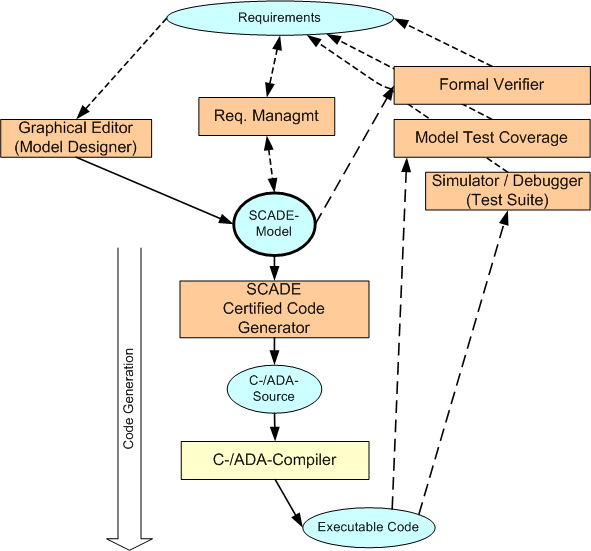
\includegraphics[scale=0.6]{SCADE_Overview.png}
\caption{SCADE Suite Overview}
\label{fig:SCADE_Suite_Overview}
\end{figure}

	%Applicability
	
SCADE is a formal modelling language targeted for safety-critical embedded control applications in the avionics, rail, automotive and industrial automation domain. SCADE source code can be written as text (for anyone who likes writing plain text) or (more usual) as schematic diagrams. SCADE models are synchronously clocked data flow and state machines, that can be nested and intermixed with each other without limitations. 
SCADE provides DO-178B- and EN50128-certified code generators producing C or ADA code as output. SCADE models are therefore concrete, deterministic, executable and verifiable; it allows the production of rapid prototype as well as of safety related target system software. 

SCADE comes with an integrated development environment (SCADE Suite IDE) including code generator, graphical simulator, model checker/prover, model test coverage analyzer, report generators, version and requirements management gateway with interfaces to various other tools like static code and timing analyzers, System/SysML modelling tools etc.. The IDE provides automatization interfaces to be controlled from external tools, and all SCADE tools itself can also be used in batch mode. In addition, plugins for Eclipse integration are available. 

The SCADE paradigm of synchronously clocked data flow and state machines works perfect for embedded control or industry automation software. It is less suitable for tasks like text processing or computer graphic applications. SCADE models do not only describe the structure of software; instead, they are the software implementation itself too. System architectures typically require a higher abstraction means of description at top level like SysML. While SysML modelling can be achieved with any SysML tools, SCADE System provides an automatic transformation from SysML to SCADE. 

For a start with SCADE a learning phase of one week should be planned.   

	\textbf{License}
	
	Commercial licenses + academic license program


	\textbf{References}

	Bibliography:
	
	\url{http://www.interested-ip.eu/}\\[4pt]
	\url{http://http://www.interested-ip.eu/final-report.html/} \\[4pt]


\section{Simulink/ Design Verifier}

	\textbf{Developer}

	Company: 

	Webside:

	Contact address:

	Other  Participators:



	\textbf{Typical applications}

	Field of usage:

	%Brief introduction to what the tool does

	%Applicability
	%Key capabilities
	Input:

	Output:

	% Main restrictions e.g. only a subset of the target language is covered

	% Manual or automated use of the tool e.g. which steps are manual and automatic in the use of the tool.

	% Expertise level e.g. which prerequisite is needed to use the tool


	Integration in a tool chain
	%Currently distributed: Yes/No
	%Underlying technologies E.g. Framework, .NET vs. Java, etc.

	%Describe equirement to install/run the tool (all that is necessary to make the tool work fine: OS, Java version, dependencies with other tools, Eclipse version, ...)


	\textbf{License}


	\textbf{References}

	Bibliography:


\section{SPARK GPL/ GNATprove}

	\textbf{Developer}

	Company: 

	Webside:

	Contact address:

	Other  Participators:



	\textbf{Typical applications}

	Field of usage:

	%Brief introduction to what the tool does

	%Applicability
	%Key capabilities
	Input:

	Output:

	% Main restrictions e.g. only a subset of the target language is covered

	% Manual or automated use of the tool e.g. which steps are manual and automatic in the use of the tool.

	% Expertise level e.g. which prerequisite is needed to use the tool


	Integration in a tool chain
	%Currently distributed: Yes/No
	%Underlying technologies E.g. Framework, .NET vs. Java, etc.

	%Describe equirement to install/run the tool (all that is necessary to make the tool work fine: OS, Java version, dependencies with other tools, Eclipse version, ...)


	\textbf{License}


	\textbf{References}

	Bibliography:


\section{SPIN}

	\textbf{Developer}

	Company: 

	Webside:

	Contact address:

	Other  Participators:



	\textbf{Typical applications}

	Field of usage:

	%Brief introduction to what the tool does

	%Applicability
	%Key capabilities
	Input:

	Output:

	% Main restrictions e.g. only a subset of the target language is covered

	% Manual or automated use of the tool e.g. which steps are manual and automatic in the use of the tool.

	% Expertise level e.g. which prerequisite is needed to use the tool


	Integration in a tool chain
	%Currently distributed: Yes/No
	%Underlying technologies E.g. Framework, .NET vs. Java, etc.

	%Describe equirement to install/run the tool (all that is necessary to make the tool work fine: OS, Java version, dependencies with other tools, Eclipse version, ...)


	\textbf{License}


	\textbf{References}

	Bibliography:


\section{$\pi$-Tool}

	\textbf{Developer}

	Company: 

	Webside:

	Contact address:

	Other  Participators:



	\textbf{Typical applications}

	Field of usage:

	%Brief introduction to what the tool does

	%Applicability
	%Key capabilities
	Input:

	Output:

	% Main restrictions e.g. only a subset of the target language is covered

	% Manual or automated use of the tool e.g. which steps are manual and automatic in the use of the tool.

	% Expertise level e.g. which prerequisite is needed to use the tool


	Integration in a tool chain
	%Currently distributed: Yes/No
	%Underlying technologies E.g. Framework, .NET vs. Java, etc.

	%Describe equirement to install/run the tool (all that is necessary to make the tool work fine: OS, Java version, dependencies with other tools, Eclipse version, ...)


	\textbf{License}


	\textbf{References}

	Bibliography:


\section{Tool chains}
As this overview only covers the most relevant tools covered during the interviews a longer list of all tools mentioned during the interviews is presented in appendix \ref{List tools}. Especially for formal proofs there is a number of tools which have been developed in academically research to check one or a group of specific properties of a certain kind of models. Most of these tools are open source. If a specific methodology has been choose it is necessary to analyse which of these tools fits the needed verification and validation activities.

Since certain methods like model-based testing include an number of different activities which are supported through different tools it is important for the development process to allow interactions between the tools. This can be the case by allowing data exchange between different tools of specified interfaces or by incorporation certain tools functionalities into a common software  environment like Eclipse. Overall all tools interaction with each other build the tool chain to support the development process. 

With TopCased and Rodin there already exist two toolchain which cover the whole software development process by using some of the tools described before. As they use the Eclipse environment other tools can be added to this toolchains. The Why3 toolchain provides a software verification platform for different theorem proofs. The following sections present an introduction for all three toolchains.

\subsection{TopCased}

	\textbf{Developer}

	Company: 

	Webside:

	Contact address:

	Other  Participators:



	\textbf{Typical applications}

	Field of usage:

	%Brief introduction to what the tool does

	%Applicability
	%Key capabilities
	Input:

	Output:

	% Main restrictions e.g. only a subset of the target language is covered

	% Manual or automated use of the tool e.g. which steps are manual and automatic in the use of the tool.

	% Expertise level e.g. which prerequisite is needed to use the tool


	Integration in a tool chain
	%Currently distributed: Yes/No
	%Underlying technologies E.g. Framework, .NET vs. Java, etc.

	%Describe equirement to install/run the tool (all that is necessary to make the tool work fine: OS, Java version, dependencies with other tools, Eclipse version, ...)


	\textbf{License}


	\textbf{References}

	Bibliography:

\subsection{Rodin}

	\textbf{Developer}

	Company: 

	Webside:

	Contact address:

	Other  Participators:



	\textbf{Typical applications}

	Field of usage:

	%Brief introduction to what the tool does

	%Applicability
	%Key capabilities
	Input:

	Output:

	% Main restrictions e.g. only a subset of the target language is covered

	% Manual or automated use of the tool e.g. which steps are manual and automatic in the use of the tool.

	% Expertise level e.g. which prerequisite is needed to use the tool


	Integration in a tool chain
	%Currently distributed: Yes/No
	%Underlying technologies E.g. Framework, .NET vs. Java, etc.

	%Describe equirement to install/run the tool (all that is necessary to make the tool work fine: OS, Java version, dependencies with other tools, Eclipse version, ...)


	\textbf{License}


	\textbf{References}

	Bibliography:

\subsection{Why3}

	\textbf{Developer}

	Company: 

	Webside:

	Contact address:

	Other  Participators:



	\textbf{Typical applications}

	Field of usage:

	%Brief introduction to what the tool does

	%Applicability
	%Key capabilities
	Input:

	Output:

	% Main restrictions e.g. only a subset of the target language is covered

	% Manual or automated use of the tool e.g. which steps are manual and automatic in the use of the tool.

	% Expertise level e.g. which prerequisite is needed to use the tool


	Integration in a tool chain
	%Currently distributed: Yes/No
	%Underlying technologies E.g. Framework, .NET vs. Java, etc.

	%Describe equirement to install/run the tool (all that is necessary to make the tool work fine: OS, Java version, dependencies with other tools, Eclipse version, ...)


	\textbf{License}


	\textbf{References}

	Bibliography:


\section{Summary}

Overall a large number of tools is available for different tasks in the software development process. Currently most companies use commercial software, but a growing number of open source software is available.  Correspondingly most interviewees reckon that open source software which is proven in use and for which a strong service support can be provided is suitable for  safety relevant software development. 

The interviews have mainly been focus on modeling tools as for verification and validation usually a combination of specified tools and tool additions is used. Artisan Studio, Atelier B, iLock, SCADE and Simulink have been the tools used by most companies for their software development. Usually these tools are  costumised to fit the needs of the individual development process and further tools are added to provide additional functionalities.

\chapter{Conclusions and Recommendations}

The existing technologies for software development in railway signaling already provide a wide range of different means of descriptions, methods and tools which can be used to handle the different steps of the software development process as it is required by the \citeauthor{EN50128:2011}. As shown in chapter \ref{chapter: MoD} usually more than one means of description is needed to capture the different levels of abstraction during the various phases of the development process. To provide the proofabilty which builds the basis for the open proof approach a formal description of all specifications is needed at one point against which the requirements can be verified and validated. 

The interviews have shown that formal, model-based development methods are already common practice for the lower abstraction levels of software architecture and design. On the high abstraction levels of  software specifications usually semi-formal means of descriptions are used, which do not allow the use of formal proof. Therefore it has to be evaluated to which extend the common formal means of description can be used to modell the textual system specifications and whether it is possible to derive the software specifications based on this description. 

As it has been shown different methods can be used to get from textual system specifications to source code. As the openETCS concept already intends to use a formal software specifications as a basis for the software generation, methods to handle these development steps have to be chosen. Thereby a method has to be picked how the textual system specifications have to be formalised. This can be done via semi-formal modells or by a direct translation. 

Corresponding with the primary development methods for the formalisation of system and software specifications, the definition of software design and architecture and source code generation, the methods for verification and validation have to be chosen. According to the open proof concept this should be able to verify certain properties on the different abstraction levels during the software development. Thereby the abstraction level on which a certain verification can be done and the method that can be used depends directly on the kind of property and the degree of formalisation on the abstraction level. Overall a consistent coordination between provided details and for verification needed information has to be established. Correspondingly it has to be defined which formal proofs or test cases can be used to validated all kind of requirements.

As most of the tools currently in use for software development are commerical products, it has to be evaluated closely which open source tools provide the needed functionality and  robustness to be incorporated in the software development. As most interviews confirmed that open source tools should be able to handle the needed development functionalities, acceptance of open source tools should not be a general barrier. 

Since a wide range of different functionalities has to be supported by tools it is necessary to find a fitting combination of tools which provide which support the selected development methods. As it can be seen at the already existing toolchains Topcased and Rodin the Eclipse framework provides a suitable basis for the tool combination. Correspondingly the interfaces between the different tools and their supported development steps have to be clearly defined to guarantee a safe data exchange.

Overall it can be seen that various means of decription, methods and tools are currently used in the signaling industry for software development, but the open proof concept of openETCS needs a more formalised development process as it exists today. Therefore it is necessary to select a more formalised  development process has to be defined which builds on the existing model-based approaches. Based on the development methods probably a combination of suitable means of description for the different abstraction levels have to be chosen from the various means of description used currently. Afterwards suitable tools which support the resulting development process and the needed means of description have to be evaluated and combined to for the integrated toolchain for the software development.

\appendix

\chapter{Questionnaire for Interviews}
\label{chap: questionnaire}

2012-07-19, V1.3 

\textbf{\Large GENERAL INFORMATION CONCERNING THE INTERVIEWS AND THIS QUESTIONAIRE}

\textbf {Attention: This is the version of the questionnaire to be answered by chosen signalling and modelling experts, once it has been agreed on. It is not to be answered by all members of WP 2.}

The model of a technical system requires a method, tools and means of description used in a certain context. In the interviews that will be performed in WP 2 of openETCS, the used methods, tools and means of description used by signalling experts in the signalling industry and beyond when modelling complex safety relevant systems will be evaluated. The methods used for formal modelling of complex technical systems will not only be evaluated in the railway domain but in other domains as well. This input from other industries shall enable the openETCS project consortium to benefit from external developments.
The evaluation carried out by the interviews will not only focus on the methods used but as well problems experts are dealing with during their daily work with formal modelling and the requested tools, methods and means of description. This will result in setting up requirements on the methods, tools and means of description to be used within openETCS. The results of the interviews will be summarised in a report.


The interview itself is intended to be carried out in a comfortable atmosphere at the premises of the participating signalling experts. The listed questions will only be a guideline, the interviews shall take place as a relaxed conversation. The target of the interviews is to have a good usable and accepted method which can be generally used to model the ETCS system.\newpage

 
{\begin{enumerate}


	\renewcommand{\theenumi}{\Alph{enumi}}
	\renewcommand{\labelenumi}{\theenumi}

	\renewcommand{\theenumii}{\arabic{enumii}}
	\renewcommand{\labelenumii}{\theenumii}

      {\Large \item Structure of your organisation}

	\begin{enumerate}

	
    	  \item Please provide an organization chart of your organisation with focus on the group working on formal modelling.
    	  \item What is the product of your company/ department formal modelling is used for?
 	  \item If a safety relevant system is modelled in your organisation, which parties and/ or groups are involved?
              \item Is there a rule for specific methods, tools and means of description to be used in your organisation?
  	  \item What would be required for a change of the methods, tools and means of description?
	  \item Which requirements have to be fulfilled by your tool and can those be met by open source solutions?
   	  \item If a technical system is modelled, how does the internal approval process work?
    	  \item Have the methods used in your organisation any normative or legal background?
    	  \item Is there a task in your development process which you would like to enhance through formal modelling?
	\end{enumerate}


     {\Large \item  Development methods}
	

	\begin{enumerate}

	 \item Which development method do you use, why?
	 \item Do your partners use the same development methods?
	 \item Have the development methods used by your partners an influence on your work?
	 \item	How do you deal with different development methods?
	 \item	How much input for a new project is normally taken from previous projects and in which format are these information usually provided?
	\end{enumerate}


  {\Large \item   Code development}



\begin{enumerate}
  \item  Is your code development model based?
  \item  Are tests included in your code development?
  \item  Do you work during your tool development with a versioning system?
  \item  Do you use a configuration management?
\end{enumerate}

  {\Large \item  Verification and Validation of models and code}

\begin{enumerate}
  \item  How is your processes structured to verify and validate models and code?
  \item  How do you create test cases for verification and validation of models and code?
  \item  Do your partners provide certain process requirements or test cases?
  \item  Are your partners involved in the whole verification and validation process?
  \item  How can you adapt your verification and validation process, if different requirements for testing have to be integrated?
\end{enumerate}

  {\Large \item   Experience with methods}

\begin{enumerate}
  \item  Are you satisfied with the methods you are using?
  \item  Which problems occur when using the methods?
\end{enumerate}


  {\Large \item  Requirement on future methods}

\begin{enumerate}
  \item  Which additive functions should modelling methods used in future in your organisation have?
  \item  Which general requirements do you have on methods?
\end{enumerate}

\end{enumerate}

\chapter{List Means of description}
\label{chap: TabMoD}

\begin{center}
   \begin{landscape}
%\begin{sidewaystable}
%\begin{table}[htp]





\begin{longtable}{|m{6cm}|m{0.8cm}|m{0.3cm}|m{0.3cm}|m{0.7cm}|m{0.3cm}|m{0.3cm}|m{0.7cm}|m{0.3cm}|m{0.3cm}|m{0.3cm}|m{0.3cm}|m{0.3cm}|m{0.7cm}|m{0.7cm}|m{0.7cm}|m{0.3cm}|}

\caption{Characterisation with detailed criterias for relevant Means of Description in basis of  VDI/VDE 3681:2005}
\label{tab:TabMoD-long}\\

\hline
 & \multicolumn{16}{|c|}{Criteria} \\ \hline
&&& \multicolumn{3}{|m{1.3cm}|}{Representation}& \multicolumn{3}{|m{1.8cm}|}{Description of structure}&\multicolumn{4}{|m{2.5cm}|}{Description of behaviour}& & & &  \\ \hline
& \rotatebox{90}{~\parbox{3cm}{MoD/ Technique} }&
\rotatebox{90}{~\parbox{3cm}{Formal basis}}& 
\rotatebox{90}{~\parbox{3cm}{Textual}}& 
\rotatebox{90}{~\parbox{3cm}{Mathematical-symbolic}}& 
\rotatebox{90}{~\parbox{3cm}{Graphical}}& 
\rotatebox{90}{~\parbox{3cm}{Hierarchical}} &
\rotatebox{90}{~\parbox{3cm}{Composition/ decomposition}} &
\rotatebox{90}{~\parbox{3cm}{Structural change}} &
\rotatebox{90}{~\parbox{3cm}{Deterministic}} &
\rotatebox{90}{~\parbox{3cm}{Non-deterministic}} &
\rotatebox{90}{~\parbox{3cm}{Static}} &
\rotatebox{90}{~\parbox{3cm}{Dynamic}} &
\rotatebox{90}{~\parbox{3cm}{Explicit time representation}} &
\rotatebox{90}{~\parbox{3cm}{No expertise required}} & 
\rotatebox{90}{~\parbox{3cm}{Level of standardization}} &
\rotatebox{90}{~\parbox{3cm}{Tool support}} \\ \hline
\endfirsthead

\hline
 & \multicolumn{16}{|c|}{Criteria} \\ \hline
&&& \multicolumn{3}{|m{1.3cm}|}{Representation}& \multicolumn{3}{|m{1.8cm}|}{Description of structure}&\multicolumn{4}{|m{2.5cm}|}{Description of behaviour}& & & &  \\ \hline
& \rotatebox{90}{~\parbox{3cm}{MoD/ Technique} }&
\rotatebox{90}{~\parbox{3cm}{Formal basis}}& 
\rotatebox{90}{~\parbox{3cm}{Textual}}& 
\rotatebox{90}{~\parbox{3cm}{Mathematical-symbolic}}& 
\rotatebox{90}{~\parbox{3cm}{Graphical}}& 
\rotatebox{90}{~\parbox{3cm}{Hierarchical}} &
\rotatebox{90}{~\parbox{3cm}{Composition/ decomposition}} &
\rotatebox{90}{~\parbox{3cm}{Structural change}} &
\rotatebox{90}{~\parbox{3cm}{Deterministic}} &
\rotatebox{90}{~\parbox{3cm}{Non-deterministic}} &
\rotatebox{90}{~\parbox{3cm}{Static}} &
\rotatebox{90}{~\parbox{3cm}{Dynamic}} &
\rotatebox{90}{~\parbox{3cm}{Explicit time representation}} &
\rotatebox{90}{~\parbox{3cm}{No expertise required}} & 
\rotatebox{90}{~\parbox{3cm}{Level of standardization}} &
\rotatebox{90}{~\parbox{3cm}{Tool support}} \\ \hline
\endhead

\multicolumn{17}{|c|}{MoD - Means of Description, Tech - Technique} \\
\multicolumn{17}{|c|}{+ - fulfills criteria completely  (can be used) , o - fulfills criteria partially (can be used to some extent), - - does not fulfills criteria (cannot be used)} \\ \hline
\multicolumn{17}{|r|}{{Overview of means of descriptions - Continued on next page}} \\ \hline
\endfoot

\multicolumn{17}{|c|}{MoD - Means of Description, Tech - Technique} \\
\multicolumn{17}{|c|}{+ - fulfills criteria completely  (can be used) , o - fulfills criteria partially (can be used to some extent), - - does not fulfills criteria (cannot be used)} \\ \hline
\endlastfoot

ACSL (ANSI/ISO C Specification Language) and C&MoD&o&+&&&+&+&-&+&-&+&+&-&-&+&+ \\ \hline
Ada and Spark&MoD&o&+&&&+&+&-&+&-&+&+&-&-&+&+ \\ \hline
Alloy&MoD&+&&+&&+&+&o&+&o&+&o&-&-&-&+ \\ \hline
CNL (Controlled Natural Language)&MoD&+&+&+&&-&-&-&+&-&+&o&-&o&-&o \\ \hline
HOL (High Order Logic)&MoD&+&&+&&+&+&o&+&+&+&o&+&-&-&o \\ \hline
Lustre / Textual and Graphical Scade&MoD&+&+&&+&+&+&+&+&+&+&+&-&-&o&+ \\ \hline
OBJ&MoD&+&&+&&+&+&-&+&-&+&o&-&&& \\ \hline
RSL (RAISE Specification Language)&MoD&+& &+& &+&+& &+& &+&+&+&-&o&+\\ \hline
Timed Petri Nets&MoD&+&o&o&+&+&+&+&+&+&+&+&+&-&+&o\\ \hline
Process Calculi (CCS, CSP, LOToS)&MoD&+&&+&&-&-&-&o&-&+&-&&&& \\ \hline
State Machines&MoD&+&&+&+&o&-&-&o&o&+&+&-&-&-&+ \\ \hline
TL (Temporal Logic)&MoD&+&&+&&-&-&-&+&o&+&+&-&-&-&o \\ \hline
UML 2.0 (Unified Modelling Language) and SysML (System Modelling Language)&MoD&o&+&&+&+&+&o&+&o&+&+&+&o&+&+ \\ \hline
VDM (Vienna Development Method)&T&+&&+&&+&+&o&+&&+&o&-&-&+&+ \\ \hline
Z, B - Method and Event B&T&+&&+&o&+&+&o&+&o&+&+&o&-&+&+ \\ \hline


\end{longtable}
%\end{table}

%\end{sidewaystable}
   \end{landscape}
\end{center}

\begin{tabbing}





\end{tabbing}

\chapter{Recommended methods}
\label{chap: method}



\begin{longtable}{|m{4cm}|p{3.5cm}|m{0.6cm}|m{0.6cm}|m{0.3cm}|m{0.6cm}|m{0.3cm}|m{0.3cm}|m{0.6cm}|}

\caption{Overview of methods and their associated development phases}
\label{tab: methods}\\

\hline \rotatebox{90}{~\parbox{5cm}{\textbf{Method}}}&  & 
\rotatebox{90}{~\parbox{5cm}{\textbf{Trans. of text. specs in formal specs}}}
 & \rotatebox{90}{~\parbox{5cm}{\textbf{Trans. of formal requirement specs to formal software}}}
 & \rotatebox{90}{~\parbox{5cm}{\textbf{Source code generation}}}
 & \rotatebox{90}{~\parbox{5cm}{\textbf{Verification of models and source code}}}
 & \rotatebox{90}{~\parbox{5cm}{\textbf{Validation}} }
& \rotatebox{90}{~\parbox{5cm}{\textbf{Creation of documentation}}}
 & \rotatebox{90}{~\parbox{5cm}{\textbf{Terminology management/ Intelligent Glossary}}}
\\ \hline
\endfirsthead


\hline\rotatebox{90}{~\parbox{5cm}{\textbf{Method}}}&  & 
\rotatebox{90}{~\parbox{5cm}{\textbf{Trans. of text. specs in formal specs}}}
 & \rotatebox{90}{~\parbox{5cm}{\textbf{Trans. of formal requirement specs to formal software}}}
 & \rotatebox{90}{~\parbox{5cm}{\textbf{Source code generation}}}
 & \rotatebox{90}{~\parbox{5cm}{\textbf{Verification of models and source code}}}
 & \rotatebox{90}{~\parbox{5cm}{\textbf{Validation}} }
& \rotatebox{90}{~\parbox{5cm}{\textbf{Creation of documentation}}}
 & \rotatebox{90}{~\parbox{5cm}{\textbf{Terminology management/ Intelligent Glossary}}}
\\ \hline
\endhead

\multicolumn{9}{|c|}{+ - can be used , o - can be used to some extent} \\
\multicolumn{9}{|r|}{{Overview of methods and their associated development phases - Continued on next page}} \\ \hline
\endfoot

\multicolumn{9}{|c|}{+ - can be used , o - can be used to some extent} \\
 \hline
\endlastfoot

Decision Tables & & o & o & & + & + & & \\ \hline
Categorisation of requirements&&+&o&&&&&\\ \hline
\multirow{3}{4cm}{Trusted Components} &Library of Trusted/ Verified Components&+&+&+&+&+&o&o\\ \cline{2-9}
 &Tools proven in use&+&+&+&+&+&o&o\\ \cline{2-9}
 &Certified Tools and certified Translators&+&+&+&+&+&+&+\\ \hline
Configuration Management&&+&+&+&+&+&+&+\\ \hline
Traceability&&+&+&+&+&+&+&+\\ \hline
Model-based development&&+&+&+&+&+&+&+\\ \hline
Translation&&+&+&+&&&+&\\ \hline
Structured processes&&+&+&+&&&&+\\ \hline
Checklists&&+&&&+&+&+&\\ \hline
Requirement management&&+&&&&&&+\\ \hline
Linked Glossary&&+&+&&&&+&+\\ \hline
Terminology Engineering&&+&&&&&+&+\\ \hline
\multirow{3}{4cm}{Functional/Black-box Testing}&Prototyping/ Animation&+&+&o&+&+&&\\ \cline{2-9}
 &Boundary Value Analysis&&+&+&+&+&&\\ \cline{2-9}
 &Test Case Catalogue&&&&+&+&&\\ \hline
\multirow{5}{4cm}{Analysis and Testing}&Interface Testing&&o&o&+&+&&\\ \cline{2-9}
 &Stress-Testing&&&&o&+&&\\ \cline{2-9}
 &Test Oracle&&&&+&o&&\\ \cline{2-9}
 &Model-based Testing&&&&+&+&&\\ \cline{2-9}
 &Performance Testing&&&&+&+&&\\ \hline
\multirow{3}{4cm}{Error Avoiding Methods}&Error Detecting and Correcting Codes&&o&o&+&&&\\ \cline{2-9}
 &Error Guessing&&o&o&+&&&\\ \cline{2-9}
 &Error Seeding&&o&o&+&&&\\ \hline
Modular Approach&&&+&+&+&&&\\ \hline
Interpretation&&&+&+&&&+&\\ \hline
Dynamic Reconfigurtation&&&+&&&&&\\ \hline
Formal Refinement&&&+&&&&&\\ \hline
\multirow{3}{4cm}{Design Analysis}& Design Constraint Analysis&&&o&+&o&&\\ \cline{2-9}
 &Design Interface Analysis&&&o&+&o&&\\ \cline{2-9}
 &Design Logic Analysis&&&o&+&o&&\\ \hline
\multirow{3}{4cm}{Formal Proof}&Theorem Proofing&&&&+&+&&\\ \cline{2-9}
 &Modelchecking&&&&+&+&&\\ \cline{2-9} 
 &Process Simulation&+&+&+&+&+&&\\ \hline

\end{longtable}




\chapter{List Tools}


\bibliographystyle{plainnat}
\bibliography{./ref/dkn_2012-12-23_report-wp2-t2-1-1_12_jw}




%===================================================
%Do NOT change anything below this line

\end{document}
